
% Default to the notebook output style

    


% Inherit from the specified cell style.




    
\documentclass[11pt]{article}

    
    
    \usepackage[T1]{fontenc}
    % Nicer default font (+ math font) than Computer Modern for most use cases
    \usepackage{mathpazo}

    % Basic figure setup, for now with no caption control since it's done
    % automatically by Pandoc (which extracts ![](path) syntax from Markdown).
    \usepackage{graphicx}
    % We will generate all images so they have a width \maxwidth. This means
    % that they will get their normal width if they fit onto the page, but
    % are scaled down if they would overflow the margins.
    \makeatletter
    \def\maxwidth{\ifdim\Gin@nat@width>\linewidth\linewidth
    \else\Gin@nat@width\fi}
    \makeatother
    \let\Oldincludegraphics\includegraphics
    % Set max figure width to be 80% of text width, for now hardcoded.
    \renewcommand{\includegraphics}[1]{\Oldincludegraphics[width=.8\maxwidth]{#1}}
    % Ensure that by default, figures have no caption (until we provide a
    % proper Figure object with a Caption API and a way to capture that
    % in the conversion process - todo).
    \usepackage{caption}
    \DeclareCaptionLabelFormat{nolabel}{}
    \captionsetup{labelformat=nolabel}

    \usepackage{adjustbox} % Used to constrain images to a maximum size 
    \usepackage{xcolor} % Allow colors to be defined
    \usepackage{enumerate} % Needed for markdown enumerations to work
    \usepackage{geometry} % Used to adjust the document margins
    \usepackage{amsmath} % Equations
    \usepackage{amssymb} % Equations
    \usepackage{textcomp} % defines textquotesingle
    % Hack from http://tex.stackexchange.com/a/47451/13684:
    \AtBeginDocument{%
        \def\PYZsq{\textquotesingle}% Upright quotes in Pygmentized code
    }
    \usepackage{upquote} % Upright quotes for verbatim code
    \usepackage{eurosym} % defines \euro
    \usepackage[mathletters]{ucs} % Extended unicode (utf-8) support
    \usepackage[utf8x]{inputenc} % Allow utf-8 characters in the tex document
    \usepackage{fancyvrb} % verbatim replacement that allows latex
    \usepackage{grffile} % extends the file name processing of package graphics 
                         % to support a larger range 
    % The hyperref package gives us a pdf with properly built
    % internal navigation ('pdf bookmarks' for the table of contents,
    % internal cross-reference links, web links for URLs, etc.)
    \usepackage{hyperref}
    \usepackage{longtable} % longtable support required by pandoc >1.10
    \usepackage{booktabs}  % table support for pandoc > 1.12.2
    \usepackage[inline]{enumitem} % IRkernel/repr support (it uses the enumerate* environment)
    \usepackage[normalem]{ulem} % ulem is needed to support strikethroughs (\sout)
                                % normalem makes italics be italics, not underlines
    

    
    
    % Colors for the hyperref package
    \definecolor{urlcolor}{rgb}{0,.145,.698}
    \definecolor{linkcolor}{rgb}{.71,0.21,0.01}
    \definecolor{citecolor}{rgb}{.12,.54,.11}

    % ANSI colors
    \definecolor{ansi-black}{HTML}{3E424D}
    \definecolor{ansi-black-intense}{HTML}{282C36}
    \definecolor{ansi-red}{HTML}{E75C58}
    \definecolor{ansi-red-intense}{HTML}{B22B31}
    \definecolor{ansi-green}{HTML}{00A250}
    \definecolor{ansi-green-intense}{HTML}{007427}
    \definecolor{ansi-yellow}{HTML}{DDB62B}
    \definecolor{ansi-yellow-intense}{HTML}{B27D12}
    \definecolor{ansi-blue}{HTML}{208FFB}
    \definecolor{ansi-blue-intense}{HTML}{0065CA}
    \definecolor{ansi-magenta}{HTML}{D160C4}
    \definecolor{ansi-magenta-intense}{HTML}{A03196}
    \definecolor{ansi-cyan}{HTML}{60C6C8}
    \definecolor{ansi-cyan-intense}{HTML}{258F8F}
    \definecolor{ansi-white}{HTML}{C5C1B4}
    \definecolor{ansi-white-intense}{HTML}{A1A6B2}

    % commands and environments needed by pandoc snippets
    % extracted from the output of `pandoc -s`
    \providecommand{\tightlist}{%
      \setlength{\itemsep}{0pt}\setlength{\parskip}{0pt}}
    \DefineVerbatimEnvironment{Highlighting}{Verbatim}{commandchars=\\\{\}}
    % Add ',fontsize=\small' for more characters per line
    \newenvironment{Shaded}{}{}
    \newcommand{\KeywordTok}[1]{\textcolor[rgb]{0.00,0.44,0.13}{\textbf{{#1}}}}
    \newcommand{\DataTypeTok}[1]{\textcolor[rgb]{0.56,0.13,0.00}{{#1}}}
    \newcommand{\DecValTok}[1]{\textcolor[rgb]{0.25,0.63,0.44}{{#1}}}
    \newcommand{\BaseNTok}[1]{\textcolor[rgb]{0.25,0.63,0.44}{{#1}}}
    \newcommand{\FloatTok}[1]{\textcolor[rgb]{0.25,0.63,0.44}{{#1}}}
    \newcommand{\CharTok}[1]{\textcolor[rgb]{0.25,0.44,0.63}{{#1}}}
    \newcommand{\StringTok}[1]{\textcolor[rgb]{0.25,0.44,0.63}{{#1}}}
    \newcommand{\CommentTok}[1]{\textcolor[rgb]{0.38,0.63,0.69}{\textit{{#1}}}}
    \newcommand{\OtherTok}[1]{\textcolor[rgb]{0.00,0.44,0.13}{{#1}}}
    \newcommand{\AlertTok}[1]{\textcolor[rgb]{1.00,0.00,0.00}{\textbf{{#1}}}}
    \newcommand{\FunctionTok}[1]{\textcolor[rgb]{0.02,0.16,0.49}{{#1}}}
    \newcommand{\RegionMarkerTok}[1]{{#1}}
    \newcommand{\ErrorTok}[1]{\textcolor[rgb]{1.00,0.00,0.00}{\textbf{{#1}}}}
    \newcommand{\NormalTok}[1]{{#1}}
    
    % Additional commands for more recent versions of Pandoc
    \newcommand{\ConstantTok}[1]{\textcolor[rgb]{0.53,0.00,0.00}{{#1}}}
    \newcommand{\SpecialCharTok}[1]{\textcolor[rgb]{0.25,0.44,0.63}{{#1}}}
    \newcommand{\VerbatimStringTok}[1]{\textcolor[rgb]{0.25,0.44,0.63}{{#1}}}
    \newcommand{\SpecialStringTok}[1]{\textcolor[rgb]{0.73,0.40,0.53}{{#1}}}
    \newcommand{\ImportTok}[1]{{#1}}
    \newcommand{\DocumentationTok}[1]{\textcolor[rgb]{0.73,0.13,0.13}{\textit{{#1}}}}
    \newcommand{\AnnotationTok}[1]{\textcolor[rgb]{0.38,0.63,0.69}{\textbf{\textit{{#1}}}}}
    \newcommand{\CommentVarTok}[1]{\textcolor[rgb]{0.38,0.63,0.69}{\textbf{\textit{{#1}}}}}
    \newcommand{\VariableTok}[1]{\textcolor[rgb]{0.10,0.09,0.49}{{#1}}}
    \newcommand{\ControlFlowTok}[1]{\textcolor[rgb]{0.00,0.44,0.13}{\textbf{{#1}}}}
    \newcommand{\OperatorTok}[1]{\textcolor[rgb]{0.40,0.40,0.40}{{#1}}}
    \newcommand{\BuiltInTok}[1]{{#1}}
    \newcommand{\ExtensionTok}[1]{{#1}}
    \newcommand{\PreprocessorTok}[1]{\textcolor[rgb]{0.74,0.48,0.00}{{#1}}}
    \newcommand{\AttributeTok}[1]{\textcolor[rgb]{0.49,0.56,0.16}{{#1}}}
    \newcommand{\InformationTok}[1]{\textcolor[rgb]{0.38,0.63,0.69}{\textbf{\textit{{#1}}}}}
    \newcommand{\WarningTok}[1]{\textcolor[rgb]{0.38,0.63,0.69}{\textbf{\textit{{#1}}}}}
    
    
    % Define a nice break command that doesn't care if a line doesn't already
    % exist.
    \def\br{\hspace*{\fill} \\* }
    % Math Jax compatability definitions
    \def\gt{>}
    \def\lt{<}
    % Document parameters
    \title{hw3}
    
    
    

    % Pygments definitions
    
\makeatletter
\def\PY@reset{\let\PY@it=\relax \let\PY@bf=\relax%
    \let\PY@ul=\relax \let\PY@tc=\relax%
    \let\PY@bc=\relax \let\PY@ff=\relax}
\def\PY@tok#1{\csname PY@tok@#1\endcsname}
\def\PY@toks#1+{\ifx\relax#1\empty\else%
    \PY@tok{#1}\expandafter\PY@toks\fi}
\def\PY@do#1{\PY@bc{\PY@tc{\PY@ul{%
    \PY@it{\PY@bf{\PY@ff{#1}}}}}}}
\def\PY#1#2{\PY@reset\PY@toks#1+\relax+\PY@do{#2}}

\expandafter\def\csname PY@tok@w\endcsname{\def\PY@tc##1{\textcolor[rgb]{0.73,0.73,0.73}{##1}}}
\expandafter\def\csname PY@tok@c\endcsname{\let\PY@it=\textit\def\PY@tc##1{\textcolor[rgb]{0.25,0.50,0.50}{##1}}}
\expandafter\def\csname PY@tok@cp\endcsname{\def\PY@tc##1{\textcolor[rgb]{0.74,0.48,0.00}{##1}}}
\expandafter\def\csname PY@tok@k\endcsname{\let\PY@bf=\textbf\def\PY@tc##1{\textcolor[rgb]{0.00,0.50,0.00}{##1}}}
\expandafter\def\csname PY@tok@kp\endcsname{\def\PY@tc##1{\textcolor[rgb]{0.00,0.50,0.00}{##1}}}
\expandafter\def\csname PY@tok@kt\endcsname{\def\PY@tc##1{\textcolor[rgb]{0.69,0.00,0.25}{##1}}}
\expandafter\def\csname PY@tok@o\endcsname{\def\PY@tc##1{\textcolor[rgb]{0.40,0.40,0.40}{##1}}}
\expandafter\def\csname PY@tok@ow\endcsname{\let\PY@bf=\textbf\def\PY@tc##1{\textcolor[rgb]{0.67,0.13,1.00}{##1}}}
\expandafter\def\csname PY@tok@nb\endcsname{\def\PY@tc##1{\textcolor[rgb]{0.00,0.50,0.00}{##1}}}
\expandafter\def\csname PY@tok@nf\endcsname{\def\PY@tc##1{\textcolor[rgb]{0.00,0.00,1.00}{##1}}}
\expandafter\def\csname PY@tok@nc\endcsname{\let\PY@bf=\textbf\def\PY@tc##1{\textcolor[rgb]{0.00,0.00,1.00}{##1}}}
\expandafter\def\csname PY@tok@nn\endcsname{\let\PY@bf=\textbf\def\PY@tc##1{\textcolor[rgb]{0.00,0.00,1.00}{##1}}}
\expandafter\def\csname PY@tok@ne\endcsname{\let\PY@bf=\textbf\def\PY@tc##1{\textcolor[rgb]{0.82,0.25,0.23}{##1}}}
\expandafter\def\csname PY@tok@nv\endcsname{\def\PY@tc##1{\textcolor[rgb]{0.10,0.09,0.49}{##1}}}
\expandafter\def\csname PY@tok@no\endcsname{\def\PY@tc##1{\textcolor[rgb]{0.53,0.00,0.00}{##1}}}
\expandafter\def\csname PY@tok@nl\endcsname{\def\PY@tc##1{\textcolor[rgb]{0.63,0.63,0.00}{##1}}}
\expandafter\def\csname PY@tok@ni\endcsname{\let\PY@bf=\textbf\def\PY@tc##1{\textcolor[rgb]{0.60,0.60,0.60}{##1}}}
\expandafter\def\csname PY@tok@na\endcsname{\def\PY@tc##1{\textcolor[rgb]{0.49,0.56,0.16}{##1}}}
\expandafter\def\csname PY@tok@nt\endcsname{\let\PY@bf=\textbf\def\PY@tc##1{\textcolor[rgb]{0.00,0.50,0.00}{##1}}}
\expandafter\def\csname PY@tok@nd\endcsname{\def\PY@tc##1{\textcolor[rgb]{0.67,0.13,1.00}{##1}}}
\expandafter\def\csname PY@tok@s\endcsname{\def\PY@tc##1{\textcolor[rgb]{0.73,0.13,0.13}{##1}}}
\expandafter\def\csname PY@tok@sd\endcsname{\let\PY@it=\textit\def\PY@tc##1{\textcolor[rgb]{0.73,0.13,0.13}{##1}}}
\expandafter\def\csname PY@tok@si\endcsname{\let\PY@bf=\textbf\def\PY@tc##1{\textcolor[rgb]{0.73,0.40,0.53}{##1}}}
\expandafter\def\csname PY@tok@se\endcsname{\let\PY@bf=\textbf\def\PY@tc##1{\textcolor[rgb]{0.73,0.40,0.13}{##1}}}
\expandafter\def\csname PY@tok@sr\endcsname{\def\PY@tc##1{\textcolor[rgb]{0.73,0.40,0.53}{##1}}}
\expandafter\def\csname PY@tok@ss\endcsname{\def\PY@tc##1{\textcolor[rgb]{0.10,0.09,0.49}{##1}}}
\expandafter\def\csname PY@tok@sx\endcsname{\def\PY@tc##1{\textcolor[rgb]{0.00,0.50,0.00}{##1}}}
\expandafter\def\csname PY@tok@m\endcsname{\def\PY@tc##1{\textcolor[rgb]{0.40,0.40,0.40}{##1}}}
\expandafter\def\csname PY@tok@gh\endcsname{\let\PY@bf=\textbf\def\PY@tc##1{\textcolor[rgb]{0.00,0.00,0.50}{##1}}}
\expandafter\def\csname PY@tok@gu\endcsname{\let\PY@bf=\textbf\def\PY@tc##1{\textcolor[rgb]{0.50,0.00,0.50}{##1}}}
\expandafter\def\csname PY@tok@gd\endcsname{\def\PY@tc##1{\textcolor[rgb]{0.63,0.00,0.00}{##1}}}
\expandafter\def\csname PY@tok@gi\endcsname{\def\PY@tc##1{\textcolor[rgb]{0.00,0.63,0.00}{##1}}}
\expandafter\def\csname PY@tok@gr\endcsname{\def\PY@tc##1{\textcolor[rgb]{1.00,0.00,0.00}{##1}}}
\expandafter\def\csname PY@tok@ge\endcsname{\let\PY@it=\textit}
\expandafter\def\csname PY@tok@gs\endcsname{\let\PY@bf=\textbf}
\expandafter\def\csname PY@tok@gp\endcsname{\let\PY@bf=\textbf\def\PY@tc##1{\textcolor[rgb]{0.00,0.00,0.50}{##1}}}
\expandafter\def\csname PY@tok@go\endcsname{\def\PY@tc##1{\textcolor[rgb]{0.53,0.53,0.53}{##1}}}
\expandafter\def\csname PY@tok@gt\endcsname{\def\PY@tc##1{\textcolor[rgb]{0.00,0.27,0.87}{##1}}}
\expandafter\def\csname PY@tok@err\endcsname{\def\PY@bc##1{\setlength{\fboxsep}{0pt}\fcolorbox[rgb]{1.00,0.00,0.00}{1,1,1}{\strut ##1}}}
\expandafter\def\csname PY@tok@kc\endcsname{\let\PY@bf=\textbf\def\PY@tc##1{\textcolor[rgb]{0.00,0.50,0.00}{##1}}}
\expandafter\def\csname PY@tok@kd\endcsname{\let\PY@bf=\textbf\def\PY@tc##1{\textcolor[rgb]{0.00,0.50,0.00}{##1}}}
\expandafter\def\csname PY@tok@kn\endcsname{\let\PY@bf=\textbf\def\PY@tc##1{\textcolor[rgb]{0.00,0.50,0.00}{##1}}}
\expandafter\def\csname PY@tok@kr\endcsname{\let\PY@bf=\textbf\def\PY@tc##1{\textcolor[rgb]{0.00,0.50,0.00}{##1}}}
\expandafter\def\csname PY@tok@bp\endcsname{\def\PY@tc##1{\textcolor[rgb]{0.00,0.50,0.00}{##1}}}
\expandafter\def\csname PY@tok@fm\endcsname{\def\PY@tc##1{\textcolor[rgb]{0.00,0.00,1.00}{##1}}}
\expandafter\def\csname PY@tok@vc\endcsname{\def\PY@tc##1{\textcolor[rgb]{0.10,0.09,0.49}{##1}}}
\expandafter\def\csname PY@tok@vg\endcsname{\def\PY@tc##1{\textcolor[rgb]{0.10,0.09,0.49}{##1}}}
\expandafter\def\csname PY@tok@vi\endcsname{\def\PY@tc##1{\textcolor[rgb]{0.10,0.09,0.49}{##1}}}
\expandafter\def\csname PY@tok@vm\endcsname{\def\PY@tc##1{\textcolor[rgb]{0.10,0.09,0.49}{##1}}}
\expandafter\def\csname PY@tok@sa\endcsname{\def\PY@tc##1{\textcolor[rgb]{0.73,0.13,0.13}{##1}}}
\expandafter\def\csname PY@tok@sb\endcsname{\def\PY@tc##1{\textcolor[rgb]{0.73,0.13,0.13}{##1}}}
\expandafter\def\csname PY@tok@sc\endcsname{\def\PY@tc##1{\textcolor[rgb]{0.73,0.13,0.13}{##1}}}
\expandafter\def\csname PY@tok@dl\endcsname{\def\PY@tc##1{\textcolor[rgb]{0.73,0.13,0.13}{##1}}}
\expandafter\def\csname PY@tok@s2\endcsname{\def\PY@tc##1{\textcolor[rgb]{0.73,0.13,0.13}{##1}}}
\expandafter\def\csname PY@tok@sh\endcsname{\def\PY@tc##1{\textcolor[rgb]{0.73,0.13,0.13}{##1}}}
\expandafter\def\csname PY@tok@s1\endcsname{\def\PY@tc##1{\textcolor[rgb]{0.73,0.13,0.13}{##1}}}
\expandafter\def\csname PY@tok@mb\endcsname{\def\PY@tc##1{\textcolor[rgb]{0.40,0.40,0.40}{##1}}}
\expandafter\def\csname PY@tok@mf\endcsname{\def\PY@tc##1{\textcolor[rgb]{0.40,0.40,0.40}{##1}}}
\expandafter\def\csname PY@tok@mh\endcsname{\def\PY@tc##1{\textcolor[rgb]{0.40,0.40,0.40}{##1}}}
\expandafter\def\csname PY@tok@mi\endcsname{\def\PY@tc##1{\textcolor[rgb]{0.40,0.40,0.40}{##1}}}
\expandafter\def\csname PY@tok@il\endcsname{\def\PY@tc##1{\textcolor[rgb]{0.40,0.40,0.40}{##1}}}
\expandafter\def\csname PY@tok@mo\endcsname{\def\PY@tc##1{\textcolor[rgb]{0.40,0.40,0.40}{##1}}}
\expandafter\def\csname PY@tok@ch\endcsname{\let\PY@it=\textit\def\PY@tc##1{\textcolor[rgb]{0.25,0.50,0.50}{##1}}}
\expandafter\def\csname PY@tok@cm\endcsname{\let\PY@it=\textit\def\PY@tc##1{\textcolor[rgb]{0.25,0.50,0.50}{##1}}}
\expandafter\def\csname PY@tok@cpf\endcsname{\let\PY@it=\textit\def\PY@tc##1{\textcolor[rgb]{0.25,0.50,0.50}{##1}}}
\expandafter\def\csname PY@tok@c1\endcsname{\let\PY@it=\textit\def\PY@tc##1{\textcolor[rgb]{0.25,0.50,0.50}{##1}}}
\expandafter\def\csname PY@tok@cs\endcsname{\let\PY@it=\textit\def\PY@tc##1{\textcolor[rgb]{0.25,0.50,0.50}{##1}}}

\def\PYZbs{\char`\\}
\def\PYZus{\char`\_}
\def\PYZob{\char`\{}
\def\PYZcb{\char`\}}
\def\PYZca{\char`\^}
\def\PYZam{\char`\&}
\def\PYZlt{\char`\<}
\def\PYZgt{\char`\>}
\def\PYZsh{\char`\#}
\def\PYZpc{\char`\%}
\def\PYZdl{\char`\$}
\def\PYZhy{\char`\-}
\def\PYZsq{\char`\'}
\def\PYZdq{\char`\"}
\def\PYZti{\char`\~}
% for compatibility with earlier versions
\def\PYZat{@}
\def\PYZlb{[}
\def\PYZrb{]}
\makeatother


    % Exact colors from NB
    \definecolor{incolor}{rgb}{0.0, 0.0, 0.5}
    \definecolor{outcolor}{rgb}{0.545, 0.0, 0.0}



    
    % Prevent overflowing lines due to hard-to-break entities
    \sloppy 
    % Setup hyperref package
    \hypersetup{
      breaklinks=true,  % so long urls are correctly broken across lines
      colorlinks=true,
      urlcolor=urlcolor,
      linkcolor=linkcolor,
      citecolor=citecolor,
      }
    % Slightly bigger margins than the latex defaults
    
    \geometry{verbose,tmargin=1in,bmargin=1in,lmargin=1in,rmargin=1in}
    
    

    \begin{document}
    
    
    \maketitle
    
    

    
    \section{Homework 3: Loss
Minimization}\label{homework-3-loss-minimization}

\subsection{Modeling, Estimation and Gradient
Descent}\label{modeling-estimation-and-gradient-descent}

\subsection{Due Date: Tuesday 10/9, 11:59
PM}\label{due-date-tuesday-109-1159-pm}

\subsection{Course Policies}\label{course-policies}

Here are some important course policies. These are also located at
http://www.ds100.org/fa18/.

\textbf{Collaboration Policy}

Data science is a collaborative activity. While you may talk with others
about the homework, we ask that you \textbf{write your solutions
individually}. If you do discuss the assignments with others please
\textbf{include their names} at the top of your solution.

\subsection{This Assignment}\label{this-assignment}

In this homework, we explore modeling data, estimating optimal
parameters and a numerical estimation method, gradient descent. These
concepts are some of the fundamentals of data science and machine
learning and will serve as the building blocks for future projects,
classes, and work.

After this homework, you should feel comfortable with the following:

\begin{itemize}
\item
  Practice reasoning about a model
\item
  Build some intuition for loss functions and how they behave
\item
  Work through deriving the gradient of a loss with respect to model
  parameters
\item
  Work through a basic version of gradient descent.
\end{itemize}

This homework is comprised of completing code, deriving analytic
solutions, writing LaTex and visualizing loss.

\subsection{Submission - IMPORTANT, PLEASE
READ}\label{submission---important-please-read}

For this assignment and future assignments (homework and projects) you
will also submit your free response and plotting questions to
gradescope. To do this, you can download as PDF
(\texttt{File-\textgreater{}Download\ As-\textgreater{}PDF\ via\ Latex\ (.pdf)}).
You are responsible for submitting and tagging your answers in
gradescope. For each free response and plotting question, please
include:

\begin{enumerate}
\def\labelenumi{\arabic{enumi}.}
\tightlist
\item
  Relevant code used to generate the plot or inform your insights
\item
  The written free response or plot
\end{enumerate}

We are doing this to make it easier on our graders and for you, in the
case you need to submit a regrade request. Gradescope (as of now) is
still better for manual grading.

\subsection{Score breakdown}\label{score-breakdown}

\begin{longtable}[]{@{}ll@{}}
\toprule
Question & Points\tabularnewline
\midrule
\endhead
Question 1a & 1\tabularnewline
Question 1b & 1\tabularnewline
Question 1c & 1\tabularnewline
Question 1d & 1\tabularnewline
Question 1e & 1\tabularnewline
Question 2a & 2\tabularnewline
Question 2b & 1\tabularnewline
Question 2c & 1\tabularnewline
Question 2d & 1\tabularnewline
Question 2e & 1\tabularnewline
Question 2f & 1\tabularnewline
Question 3a & 1\tabularnewline
Question 3b & 3\tabularnewline
Question 3c & 2\tabularnewline
Question 4a & 3\tabularnewline
Question 4b & 1\tabularnewline
Question 4c & 1\tabularnewline
Question 4d & 1\tabularnewline
Question 4e & 1\tabularnewline
Question 5a & 2\tabularnewline
Question 5b & 4\tabularnewline
Question 5c & 0\tabularnewline
Question 5d & 0\tabularnewline
Question 6a & 3\tabularnewline
Question 6b & 3\tabularnewline
Question 6c & 3\tabularnewline
Question 6d & 3\tabularnewline
Question 6e & 3\tabularnewline
Question 6f & 3\tabularnewline
Question 6g & 3\tabularnewline
Question 7a & 1\tabularnewline
Question 7b & 1\tabularnewline
Question 7c & 1\tabularnewline
Question 7d & 1\tabularnewline
Question 7e & 0\tabularnewline
Total & 56\tabularnewline
\bottomrule
\end{longtable}

    \section{Getting Started}\label{getting-started}

    \begin{Verbatim}[commandchars=\\\{\}]
{\color{incolor}In [{\color{incolor}1}]:} \PY{c+c1}{\PYZsh{} Imports}
        \PY{k+kn}{import} \PY{n+nn}{pandas} \PY{k}{as} \PY{n+nn}{pd}
        \PY{k+kn}{import} \PY{n+nn}{numpy} \PY{k}{as} \PY{n+nn}{np}
        \PY{k+kn}{import} \PY{n+nn}{matplotlib}\PY{n+nn}{.}\PY{n+nn}{pyplot} \PY{k}{as} \PY{n+nn}{plt}
        \PY{k+kn}{import} \PY{n+nn}{csv}
        \PY{k+kn}{import} \PY{n+nn}{re}
        \PY{k+kn}{import} \PY{n+nn}{seaborn} \PY{k}{as} \PY{n+nn}{sns}
        
        \PY{c+c1}{\PYZsh{} Set some parameters}
        \PY{n}{plt}\PY{o}{.}\PY{n}{rcParams}\PY{p}{[}\PY{l+s+s1}{\PYZsq{}}\PY{l+s+s1}{figure.figsize}\PY{l+s+s1}{\PYZsq{}}\PY{p}{]} \PY{o}{=} \PY{p}{(}\PY{l+m+mi}{12}\PY{p}{,} \PY{l+m+mi}{9}\PY{p}{)}
        \PY{n}{plt}\PY{o}{.}\PY{n}{rcParams}\PY{p}{[}\PY{l+s+s1}{\PYZsq{}}\PY{l+s+s1}{font.size}\PY{l+s+s1}{\PYZsq{}}\PY{p}{]} \PY{o}{=} \PY{l+m+mi}{16}
        \PY{n}{np}\PY{o}{.}\PY{n}{set\PYZus{}printoptions}\PY{p}{(}\PY{l+m+mi}{4}\PY{p}{)}
\end{Verbatim}


    \begin{Verbatim}[commandchars=\\\{\}]
{\color{incolor}In [{\color{incolor}2}]:} \PY{c+c1}{\PYZsh{} We will use plot\PYZus{}3d helper function to help us visualize gradient}
        \PY{k+kn}{from} \PY{n+nn}{hw3\PYZus{}utils} \PY{k}{import} \PY{n}{plot\PYZus{}3d}
\end{Verbatim}


    \subsection{Load Data}\label{load-data}

Load the data.csv file into a pandas dataframe.\\
Note that we are reading the data directly from the URL address.

    \begin{Verbatim}[commandchars=\\\{\}]
{\color{incolor}In [{\color{incolor}3}]:} \PY{c+c1}{\PYZsh{} Run this cell to load our sample data}
        \PY{n}{data} \PY{o}{=} \PY{n}{pd}\PY{o}{.}\PY{n}{read\PYZus{}csv}\PY{p}{(}\PY{l+s+s2}{\PYZdq{}}\PY{l+s+s2}{https://github.com/DS\PYZhy{}100/fa18/raw/gh\PYZhy{}pages/assets/datasets/hw3\PYZus{}data.csv}\PY{l+s+s2}{\PYZdq{}}\PY{p}{,} \PY{n}{index\PYZus{}col}\PY{o}{=}\PY{l+m+mi}{0}\PY{p}{)}
        \PY{n}{data}\PY{o}{.}\PY{n}{head}\PY{p}{(}\PY{p}{)}
\end{Verbatim}


\begin{Verbatim}[commandchars=\\\{\}]
{\color{outcolor}Out[{\color{outcolor}3}]:}           x         y
        0 -5.000000 -7.672309
        1 -4.966555 -7.779735
        2 -4.933110 -7.995938
        3 -4.899666 -8.197059
        4 -4.866221 -8.183883
\end{Verbatim}
            
    \begin{center}\rule{0.5\linewidth}{\linethickness}\end{center}

\subsection{1: A Simple Model}\label{a-simple-model}

Let's start by examining our data and creating a simple model that can
represent this data.

    \subsubsection{Question 1}\label{question-1}

\paragraph{Question 1a}\label{question-1a}

First, let's visualize the data in a scatter plot. After implementing
the \texttt{scatter} function below, you should see something like this:
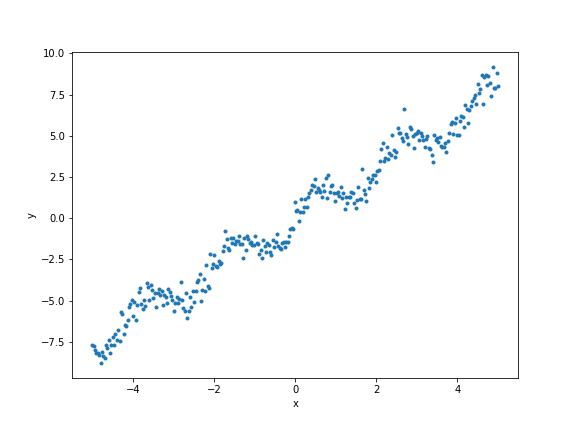
\includegraphics{scatter.png}

    \begin{Verbatim}[commandchars=\\\{\}]
{\color{incolor}In [{\color{incolor}4}]:} \PY{k}{def} \PY{n+nf}{scatter}\PY{p}{(}\PY{n}{x}\PY{p}{,} \PY{n}{y}\PY{p}{)}\PY{p}{:}
            \PY{l+s+sd}{\PYZdq{}\PYZdq{}\PYZdq{}}
        \PY{l+s+sd}{    Generate a scatter plot using x and y}
        
        \PY{l+s+sd}{    Keyword arguments:}
        \PY{l+s+sd}{    x \PYZhy{}\PYZhy{} the vector of values x}
        \PY{l+s+sd}{    y \PYZhy{}\PYZhy{} the vector of values y}
        \PY{l+s+sd}{    \PYZdq{}\PYZdq{}\PYZdq{}}
            \PY{n}{plt}\PY{o}{.}\PY{n}{figure}\PY{p}{(}\PY{n}{figsize}\PY{o}{=}\PY{p}{(}\PY{l+m+mi}{8}\PY{p}{,} \PY{l+m+mi}{6}\PY{p}{)}\PY{p}{)}
            \PY{o}{.}\PY{o}{.}\PY{o}{.}
            \PY{c+c1}{\PYZsh{}\PYZsh{}\PYZsh{} BEGIN SOLUTION}
            \PY{n}{plt}\PY{o}{.}\PY{n}{scatter}\PY{p}{(}\PY{n}{x}\PY{p}{,} \PY{n}{y}\PY{p}{,} \PY{n}{marker}\PY{o}{=}\PY{l+s+s1}{\PYZsq{}}\PY{l+s+s1}{.}\PY{l+s+s1}{\PYZsq{}}\PY{p}{)}
            \PY{n}{plt}\PY{o}{.}\PY{n}{xlabel}\PY{p}{(}\PY{l+s+s1}{\PYZsq{}}\PY{l+s+s1}{x}\PY{l+s+s1}{\PYZsq{}}\PY{p}{)}
            \PY{n}{plt}\PY{o}{.}\PY{n}{ylabel}\PY{p}{(}\PY{l+s+s1}{\PYZsq{}}\PY{l+s+s1}{y}\PY{l+s+s1}{\PYZsq{}}\PY{p}{)}
            \PY{c+c1}{\PYZsh{}\PYZsh{}\PYZsh{} END SOLUTION}
        
        \PY{n}{x} \PY{o}{=} \PY{n}{data}\PY{p}{[}\PY{l+s+s1}{\PYZsq{}}\PY{l+s+s1}{x}\PY{l+s+s1}{\PYZsq{}}\PY{p}{]}
        \PY{n}{y} \PY{o}{=} \PY{n}{data}\PY{p}{[}\PY{l+s+s1}{\PYZsq{}}\PY{l+s+s1}{y}\PY{l+s+s1}{\PYZsq{}}\PY{p}{]}
        \PY{n}{scatter}\PY{p}{(}\PY{n}{x}\PY{p}{,}\PY{n}{y}\PY{p}{)}
\end{Verbatim}


    \begin{center}
    \adjustimage{max size={0.9\linewidth}{0.9\paperheight}}{output_8_0.png}
    \end{center}
    { \hspace*{\fill} \\}
    
    \paragraph{Question 1b}\label{question-1b}

Describe any significant observations about the distribution of the
data. How can you describe the relationship between \(x\) and \(y\)?

    \subsubsection{BEGIN SOLUTION}\label{begin-solution}

The data seems to follow some sort of linear model, with sinusoidal
noise.

\subsubsection{END SOLUTION}\label{end-solution}

    \paragraph{Question 1c}\label{question-1c}

The data looks roughly linear, with some extra noise. For now, let's
assume that the data follows some underlying linear model. We define the
underlying linear model that predicts the value \(y\) using the value
\(x\) as: \(f_{\theta^*}(x) = \theta^* \cdot x\)

Since we cannot find the value of the population parameter \(\theta^*\)
exactly, we will assume that our dataset approximates our population and
use our dataset to estimate \(\theta^*\). We denote our estimation with
\(\theta\), our fitted estimation with \(\hat{\theta}\), and our model
as:

\[\Large
f_{\theta}(x) = \theta \cdot x
\]

Based on this equation, define the linear model function
\texttt{linear\_model} below to estimate \(\textbf{y}\) (the
\(y\)-values) given \(\textbf{x}\) (the \(x\)-values) and \(\theta\).
This model is similar to the model you defined in Lab 5: Modeling and
Estimation.

    \begin{Verbatim}[commandchars=\\\{\}]
{\color{incolor}In [{\color{incolor}5}]:} \PY{k}{def} \PY{n+nf}{linear\PYZus{}model}\PY{p}{(}\PY{n}{x}\PY{p}{,} \PY{n}{theta}\PY{p}{)}\PY{p}{:}
            \PY{l+s+sd}{\PYZdq{}\PYZdq{}\PYZdq{}}
        \PY{l+s+sd}{    Returns the estimate of y given x and theta}
        
        \PY{l+s+sd}{    Keyword arguments:}
        \PY{l+s+sd}{    x \PYZhy{}\PYZhy{} the vector of values x}
        \PY{l+s+sd}{    theta \PYZhy{}\PYZhy{} the scalar theta}
        \PY{l+s+sd}{    \PYZdq{}\PYZdq{}\PYZdq{}}
            \PY{n}{y} \PY{o}{=} \PY{o}{.}\PY{o}{.}\PY{o}{.}
            \PY{c+c1}{\PYZsh{}\PYZsh{}\PYZsh{} BEGIN SOLUTION}
            \PY{n}{y} \PY{o}{=} \PY{n}{theta} \PY{o}{*} \PY{n}{x}
            \PY{c+c1}{\PYZsh{}\PYZsh{}\PYZsh{} END SOLUTION}
            \PY{k}{return} \PY{n}{y}
\end{Verbatim}


    \begin{Verbatim}[commandchars=\\\{\}]
{\color{incolor}In [{\color{incolor}6}]:} \PY{k}{assert} \PY{n}{linear\PYZus{}model}\PY{p}{(}\PY{l+m+mi}{0}\PY{p}{,} \PY{l+m+mi}{1}\PY{p}{)} \PY{o}{==} \PY{l+m+mi}{0}
        \PY{k}{assert} \PY{n}{linear\PYZus{}model}\PY{p}{(}\PY{l+m+mi}{10}\PY{p}{,} \PY{l+m+mi}{10}\PY{p}{)} \PY{o}{==} \PY{l+m+mi}{100}
        \PY{k}{assert} \PY{n}{np}\PY{o}{.}\PY{n}{sum}\PY{p}{(}\PY{n}{linear\PYZus{}model}\PY{p}{(}\PY{n}{np}\PY{o}{.}\PY{n}{array}\PY{p}{(}\PY{p}{[}\PY{l+m+mi}{3}\PY{p}{,} \PY{l+m+mi}{5}\PY{p}{]}\PY{p}{)}\PY{p}{,} \PY{l+m+mi}{3}\PY{p}{)}\PY{p}{)} \PY{o}{==} \PY{l+m+mi}{24}
        \PY{k}{assert} \PY{n}{linear\PYZus{}model}\PY{p}{(}\PY{n}{np}\PY{o}{.}\PY{n}{array}\PY{p}{(}\PY{p}{[}\PY{l+m+mi}{7}\PY{p}{,} \PY{l+m+mi}{8}\PY{p}{]}\PY{p}{)}\PY{p}{,} \PY{l+m+mi}{4}\PY{p}{)}\PY{o}{.}\PY{n}{mean}\PY{p}{(}\PY{p}{)} \PY{o}{==} \PY{l+m+mi}{30}
\end{Verbatim}


    \paragraph{Question 1d}\label{question-1d}

In class, we learned that the \(L^2\) (or squared) loss function is
smooth and continuous. Let's use \(L^2\) loss to evaluate our estimate
\(\theta\), which we will use later to identify an optimal \(\theta\),
represented as \(\hat{\theta}\). Define the \(L^2\) loss function
\texttt{l2\_loss} below.

    \begin{Verbatim}[commandchars=\\\{\}]
{\color{incolor}In [{\color{incolor}7}]:} \PY{k}{def} \PY{n+nf}{l2\PYZus{}loss}\PY{p}{(}\PY{n}{y}\PY{p}{,} \PY{n}{y\PYZus{}hat}\PY{p}{)}\PY{p}{:}
            \PY{l+s+sd}{\PYZdq{}\PYZdq{}\PYZdq{}}
        \PY{l+s+sd}{    Returns the average l2 loss given y and y\PYZus{}hat}
        
        \PY{l+s+sd}{    Keyword arguments:}
        \PY{l+s+sd}{    y \PYZhy{}\PYZhy{} the vector of true values y}
        \PY{l+s+sd}{    y\PYZus{}hat \PYZhy{}\PYZhy{} the vector of predicted values y\PYZus{}hat}
        \PY{l+s+sd}{    \PYZdq{}\PYZdq{}\PYZdq{}}
            \PY{o}{.}\PY{o}{.}\PY{o}{.}
            \PY{c+c1}{\PYZsh{}\PYZsh{}\PYZsh{} BEGIN SOLUTION}
            \PY{k}{return} \PY{n}{np}\PY{o}{.}\PY{n}{mean}\PY{p}{(}\PY{n}{np}\PY{o}{.}\PY{n}{square}\PY{p}{(}\PY{n}{y} \PY{o}{\PYZhy{}} \PY{n}{y\PYZus{}hat}\PY{p}{)}\PY{p}{)}
            \PY{c+c1}{\PYZsh{}\PYZsh{}\PYZsh{} END SOLUTION}
\end{Verbatim}


    \begin{Verbatim}[commandchars=\\\{\}]
{\color{incolor}In [{\color{incolor}8}]:} \PY{k}{assert} \PY{n}{l2\PYZus{}loss}\PY{p}{(}\PY{l+m+mi}{2}\PY{p}{,} \PY{l+m+mi}{1}\PY{p}{)} \PY{o}{==} \PY{l+m+mi}{1}
        \PY{k}{assert} \PY{n}{l2\PYZus{}loss}\PY{p}{(}\PY{l+m+mi}{2}\PY{p}{,} \PY{l+m+mi}{0}\PY{p}{)} \PY{o}{==} \PY{l+m+mi}{4} 
        \PY{k}{assert} \PY{n}{l2\PYZus{}loss}\PY{p}{(}\PY{l+m+mi}{5}\PY{p}{,} \PY{l+m+mi}{1}\PY{p}{)} \PY{o}{==} \PY{l+m+mi}{16}
        \PY{k}{assert} \PY{n}{l2\PYZus{}loss}\PY{p}{(}\PY{n}{np}\PY{o}{.}\PY{n}{array}\PY{p}{(}\PY{p}{[}\PY{l+m+mi}{5}\PY{p}{,} \PY{l+m+mi}{6}\PY{p}{]}\PY{p}{)}\PY{p}{,} \PY{n}{np}\PY{o}{.}\PY{n}{array}\PY{p}{(}\PY{p}{[}\PY{l+m+mi}{1}\PY{p}{,} \PY{l+m+mi}{1}\PY{p}{]}\PY{p}{)}\PY{p}{)} \PY{o}{==} \PY{l+m+mf}{20.5}
        \PY{k}{assert} \PY{n}{l2\PYZus{}loss}\PY{p}{(}\PY{n}{np}\PY{o}{.}\PY{n}{array}\PY{p}{(}\PY{p}{[}\PY{l+m+mi}{1}\PY{p}{,} \PY{l+m+mi}{1}\PY{p}{,} \PY{l+m+mi}{1}\PY{p}{]}\PY{p}{)}\PY{p}{,} \PY{n}{np}\PY{o}{.}\PY{n}{array}\PY{p}{(}\PY{p}{[}\PY{l+m+mi}{4}\PY{p}{,} \PY{l+m+mi}{1}\PY{p}{,} \PY{l+m+mi}{4}\PY{p}{]}\PY{p}{)}\PY{p}{)} \PY{o}{==} \PY{l+m+mf}{6.0}
\end{Verbatim}


    \paragraph{Question 1e}\label{question-1e}

First, visualize the \(L^2\) loss as a function of \(\theta\), where
several different values of \(\theta\) are given. Be sure to label your
axes properly. You plot should look something like this:
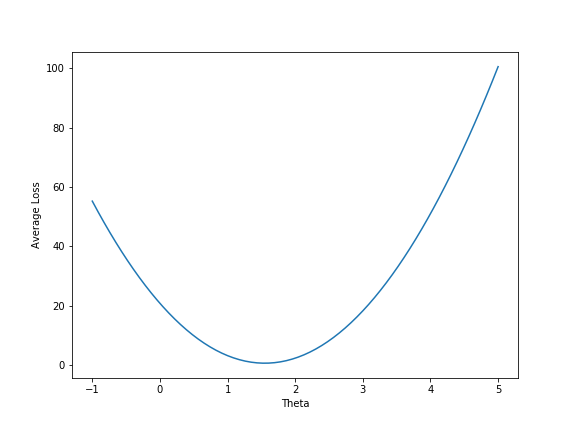
\includegraphics{l2_avg_loss.png}

What looks like the optimal value, \(\hat{\theta}\), based on the
visualization? Set \texttt{theta\_star\_guess} to the value of
\(\theta\) that appears to minimize our loss.

    \begin{Verbatim}[commandchars=\\\{\}]
{\color{incolor}In [{\color{incolor}9}]:} \PY{k}{def} \PY{n+nf}{visualize}\PY{p}{(}\PY{n}{x}\PY{p}{,} \PY{n}{y}\PY{p}{,} \PY{n}{thetas}\PY{p}{)}\PY{p}{:}
            \PY{l+s+sd}{\PYZdq{}\PYZdq{}\PYZdq{}}
        \PY{l+s+sd}{    Plots the average l2 loss for given x, y as a function of theta.}
        \PY{l+s+sd}{    Use the functions you wrote for linear\PYZus{}model and l2\PYZus{}loss.}
        
        \PY{l+s+sd}{    Keyword arguments:}
        \PY{l+s+sd}{    x \PYZhy{}\PYZhy{} the vector of values x}
        \PY{l+s+sd}{    y \PYZhy{}\PYZhy{} the vector of values y}
        \PY{l+s+sd}{    thetas \PYZhy{}\PYZhy{} an array containing different estimates of the scalar theta}
        \PY{l+s+sd}{    \PYZdq{}\PYZdq{}\PYZdq{}}
            \PY{n}{avg\PYZus{}loss} \PY{o}{=} \PY{o}{.}\PY{o}{.}\PY{o}{.} \PY{c+c1}{\PYZsh{} Calculate the loss here for each value of theta}
            
            \PY{n}{plt}\PY{o}{.}\PY{n}{figure}\PY{p}{(}\PY{n}{figsize}\PY{o}{=}\PY{p}{(}\PY{l+m+mi}{8}\PY{p}{,}\PY{l+m+mi}{6}\PY{p}{)}\PY{p}{)}
            
            \PY{o}{.}\PY{o}{.}\PY{o}{.} \PY{c+c1}{\PYZsh{} Create your plot here}
            
            \PY{c+c1}{\PYZsh{}\PYZsh{}\PYZsh{} BEGIN SOLUTION}
            \PY{n}{avg\PYZus{}loss} \PY{o}{=} \PY{n}{np}\PY{o}{.}\PY{n}{array}\PY{p}{(}\PY{p}{[}\PY{n}{l2\PYZus{}loss}\PY{p}{(}\PY{n}{linear\PYZus{}model}\PY{p}{(}\PY{n}{x}\PY{p}{,} \PY{n}{theta}\PY{p}{)}\PY{p}{,} \PY{n}{y}\PY{p}{)} \PY{k}{for} \PY{n}{theta} \PY{o+ow}{in} \PY{n}{thetas}\PY{p}{]}\PY{p}{)}
            \PY{n}{plt}\PY{o}{.}\PY{n}{plot}\PY{p}{(}\PY{n}{thetas}\PY{p}{,} \PY{n}{avg\PYZus{}loss}\PY{p}{)}
            \PY{n}{plt}\PY{o}{.}\PY{n}{xlabel}\PY{p}{(}\PY{l+s+s2}{\PYZdq{}}\PY{l+s+s2}{Theta}\PY{l+s+s2}{\PYZdq{}}\PY{p}{)}
            \PY{n}{plt}\PY{o}{.}\PY{n}{ylabel}\PY{p}{(}\PY{l+s+s2}{\PYZdq{}}\PY{l+s+s2}{Average Loss}\PY{l+s+s2}{\PYZdq{}}\PY{p}{)}
            \PY{c+c1}{\PYZsh{}\PYZsh{}\PYZsh{} END SOLUTION}
            
        \PY{n}{thetas} \PY{o}{=} \PY{n}{np}\PY{o}{.}\PY{n}{linspace}\PY{p}{(}\PY{o}{\PYZhy{}}\PY{l+m+mi}{1}\PY{p}{,} \PY{l+m+mi}{5}\PY{p}{,} \PY{l+m+mi}{70}\PY{p}{)}
        \PY{n}{visualize}\PY{p}{(}\PY{n}{x}\PY{p}{,} \PY{n}{y}\PY{p}{,} \PY{n}{thetas}\PY{p}{)}
        
        \PY{n}{theta\PYZus{}star\PYZus{}guess} \PY{o}{=} \PY{o}{.}\PY{o}{.}\PY{o}{.}
        \PY{c+c1}{\PYZsh{}\PYZsh{}\PYZsh{} BEGIN SOLUTION}
        \PY{n}{theta\PYZus{}star\PYZus{}guess} \PY{o}{=} \PY{l+m+mf}{1.5}
        \PY{c+c1}{\PYZsh{}\PYZsh{}\PYZsh{} END SOLUTION}
\end{Verbatim}


    \begin{center}
    \adjustimage{max size={0.9\linewidth}{0.9\paperheight}}{output_18_0.png}
    \end{center}
    { \hspace*{\fill} \\}
    
    \begin{Verbatim}[commandchars=\\\{\}]
{\color{incolor}In [{\color{incolor}10}]:} \PY{k}{assert} \PY{n}{l2\PYZus{}loss}\PY{p}{(}\PY{l+m+mi}{3}\PY{p}{,} \PY{l+m+mi}{2}\PY{p}{)} \PY{o}{==} \PY{l+m+mi}{1}
         \PY{k}{assert} \PY{n}{l2\PYZus{}loss}\PY{p}{(}\PY{l+m+mi}{0}\PY{p}{,} \PY{l+m+mi}{10}\PY{p}{)} \PY{o}{==} \PY{l+m+mi}{100}
         \PY{k}{assert} \PY{l+m+mi}{1} \PY{o}{\PYZlt{}}\PY{o}{=} \PY{n}{theta\PYZus{}star\PYZus{}guess} \PY{o}{\PYZlt{}}\PY{o}{=} \PY{l+m+mi}{2}
\end{Verbatim}


    \begin{center}\rule{0.5\linewidth}{\linethickness}\end{center}

\subsection{2: Fitting our Simple Model}\label{fitting-our-simple-model}

Now that we have defined a simple linear model and loss function, let's
begin working on fitting our model to the data.

\subsubsection{Question 2}\label{question-2}

Let's confirm our visual findings for optimal \(\hat{\theta}\).

\paragraph{Question 2a}\label{question-2a}

First, find the analytical solution for the optimal \(\hat{\theta}\) for
average \(L^2\) loss. Write up your solution in the cell below using
LaTex.

Hint: notice that we now have \(\textbf{x}\) and \(\textbf{y}\) instead
of \(x\) and \(y\). This means that when writing the loss function
\(L(\textbf{x}, \textbf{y}, \theta)\), you'll need to take the average
of the squared losses for each \(y_i\), \(f_\theta(x_i)\) pair. For tips
on getting started, see chapter
\href{https://www.textbook.ds100.org/ch/10/modeling_loss_functions.html}{chapter
10} of the textbook. Note that if you click "Open in DataHub", you can
access the LaTeX source code of the book chapter, which you might find
handy for typing up your work. Show your work, i.e. don't just write the
answer.

    \subsubsection{Begin Solution}\label{begin-solution}

\(\begin{align*} L(\textbf{x}, \textbf{y}, \theta) &= \frac{1}{n} \sum_{i=1}^n (\theta \cdot x_i - y_i)^2 \\ \frac{\partial L}{\partial \theta} &= \frac{2}{n} \sum_{i=1}^n (\theta \cdot x_i - y_i) \cdot x_i \\ &= \frac{2}{n} (\theta \sum_{i=1}^n x_i^2 - \sum_{i=1}^n x_i y_i) = 0 \\ \hat{\theta} &= \frac{\sum_{i=1}^n x_i y_i}{\sum_{i=1}^n x_i^2} \end{align*}\)

\subsubsection{End Solution}\label{end-solution}

    \paragraph{Question 2b}\label{question-2b}

Now that we have the analytic solution for \(\hat{\theta}\), implement
the function \texttt{find\_theta} that calculates the numerical value of
\(\hat{\theta}\) based on our data \(\textbf{x}\), \(\textbf{y}\).

    \begin{Verbatim}[commandchars=\\\{\}]
{\color{incolor}In [{\color{incolor}11}]:} \PY{k}{def} \PY{n+nf}{find\PYZus{}theta}\PY{p}{(}\PY{n}{x}\PY{p}{,} \PY{n}{y}\PY{p}{)}\PY{p}{:}
             \PY{l+s+sd}{\PYZdq{}\PYZdq{}\PYZdq{}}
         \PY{l+s+sd}{    Find optimal theta given x and y}
         
         \PY{l+s+sd}{    Keyword arguments:}
         \PY{l+s+sd}{    x \PYZhy{}\PYZhy{} the vector of values x}
         \PY{l+s+sd}{    y \PYZhy{}\PYZhy{} the vector of values y}
         \PY{l+s+sd}{    \PYZdq{}\PYZdq{}\PYZdq{}}
             \PY{n}{theta\PYZus{}opt} \PY{o}{=} \PY{o}{.}\PY{o}{.}\PY{o}{.}
             \PY{c+c1}{\PYZsh{}\PYZsh{}\PYZsh{} BEGIN SOLUTION}
             \PY{n}{theta\PYZus{}opt} \PY{o}{=} \PY{n}{np}\PY{o}{.}\PY{n}{dot}\PY{p}{(}\PY{n}{x}\PY{p}{,} \PY{n}{y}\PY{p}{)} \PY{o}{/} \PY{n}{np}\PY{o}{.}\PY{n}{dot}\PY{p}{(}\PY{n}{x}\PY{p}{,} \PY{n}{x}\PY{p}{)}
             \PY{c+c1}{\PYZsh{}\PYZsh{}\PYZsh{} END SOLUTION}
             \PY{k}{return} \PY{n}{theta\PYZus{}opt}
\end{Verbatim}


    \begin{Verbatim}[commandchars=\\\{\}]
{\color{incolor}In [{\color{incolor}12}]:} \PY{n}{t\PYZus{}hat} \PY{o}{=} \PY{n}{find\PYZus{}theta}\PY{p}{(}\PY{n}{x}\PY{p}{,} \PY{n}{y}\PY{p}{)}
         \PY{n+nb}{print}\PY{p}{(}\PY{n}{f}\PY{l+s+s1}{\PYZsq{}}\PY{l+s+s1}{theta\PYZus{}opt = }\PY{l+s+si}{\PYZob{}t\PYZus{}hat\PYZcb{}}\PY{l+s+s1}{\PYZsq{}}\PY{p}{)}
         
         \PY{k}{assert} \PY{l+m+mf}{1.4} \PY{o}{\PYZlt{}}\PY{o}{=} \PY{n}{t\PYZus{}hat} \PY{o}{\PYZlt{}}\PY{o}{=} \PY{l+m+mf}{1.6}
\end{Verbatim}


    \begin{Verbatim}[commandchars=\\\{\}]
theta\_opt = 1.550264808596222

    \end{Verbatim}

    \paragraph{Question 2c}\label{question-2c}

Now, let's plot our loss function again using the \texttt{visualize}
function. But this time, add a vertical line at the optimal value of
theta (plot the line \(x = \hat{\theta}\)). Your plot should look
something like this: 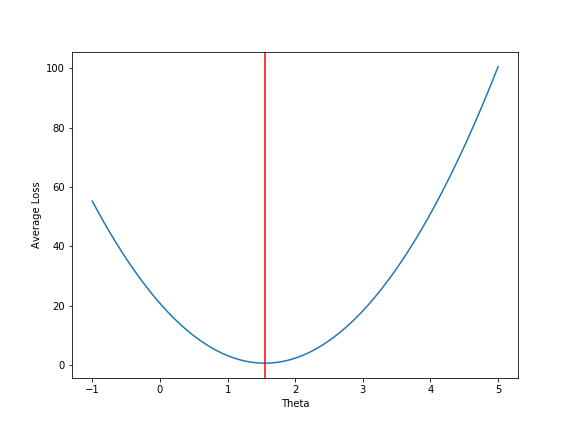
\includegraphics{vertical_linear.png}

    \begin{Verbatim}[commandchars=\\\{\}]
{\color{incolor}In [{\color{incolor}13}]:} \PY{n}{theta\PYZus{}opt} \PY{o}{=} \PY{o}{.}\PY{o}{.}\PY{o}{.}
         \PY{o}{.}\PY{o}{.}\PY{o}{.}
         \PY{o}{.}\PY{o}{.}\PY{o}{.}
         \PY{c+c1}{\PYZsh{}\PYZsh{}\PYZsh{} BEGIN SOLUTION}
         \PY{n}{theta\PYZus{}opt} \PY{o}{=} \PY{n}{find\PYZus{}theta}\PY{p}{(}\PY{n}{x}\PY{p}{,} \PY{n}{y}\PY{p}{)}
         \PY{n}{visualize}\PY{p}{(}\PY{n}{x}\PY{p}{,} \PY{n}{y}\PY{p}{,} \PY{n}{thetas}\PY{p}{)}
         \PY{n}{plt}\PY{o}{.}\PY{n}{axvline}\PY{p}{(}\PY{n}{x}\PY{o}{=}\PY{n}{theta\PYZus{}opt}\PY{p}{,} \PY{n}{color}\PY{o}{=}\PY{l+s+s1}{\PYZsq{}}\PY{l+s+s1}{r}\PY{l+s+s1}{\PYZsq{}}\PY{p}{)}
         \PY{c+c1}{\PYZsh{}\PYZsh{}\PYZsh{} END SOLUTION}
\end{Verbatim}


\begin{Verbatim}[commandchars=\\\{\}]
{\color{outcolor}Out[{\color{outcolor}13}]:} <matplotlib.lines.Line2D at 0x7f077181f4a8>
\end{Verbatim}
            
    \begin{center}
    \adjustimage{max size={0.9\linewidth}{0.9\paperheight}}{output_26_1.png}
    \end{center}
    { \hspace*{\fill} \\}
    
    \subsubsection{Question 2d}\label{question-2d}

We now have an optimal value for \(\theta\) that minimizes our loss. In
the cell below, plot the scatter plot of the data from Question 1a (you
can reuse the \texttt{scatter} function here). But this time, add the
line \(f_{\hat{\theta}}(x) = \hat{\theta} \cdot \textbf{x}\) using the
\(\hat{\theta}\) you computed above. Your plot should look something
like this: 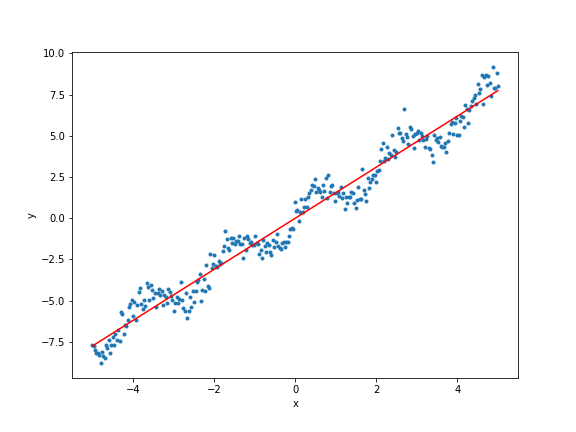
\includegraphics{scatter_with_line.png}

    \begin{Verbatim}[commandchars=\\\{\}]
{\color{incolor}In [{\color{incolor}14}]:} \PY{n}{theta\PYZus{}opt} \PY{o}{=} \PY{o}{.}\PY{o}{.}\PY{o}{.}
         \PY{o}{.}\PY{o}{.}\PY{o}{.}
         \PY{o}{.}\PY{o}{.}\PY{o}{.}
         \PY{c+c1}{\PYZsh{}\PYZsh{}\PYZsh{} BEGIN SOLUTION}
         \PY{n}{theta\PYZus{}opt} \PY{o}{=} \PY{n}{find\PYZus{}theta}\PY{p}{(}\PY{n}{x}\PY{p}{,} \PY{n}{y}\PY{p}{)}
         \PY{n}{scatter}\PY{p}{(}\PY{n}{x}\PY{p}{,} \PY{n}{y}\PY{p}{)}
         \PY{n}{line\PYZus{}values} \PY{o}{=} \PY{n}{linear\PYZus{}model}\PY{p}{(}\PY{n}{x}\PY{p}{,} \PY{n}{theta\PYZus{}opt}\PY{p}{)}
         \PY{n}{plt}\PY{o}{.}\PY{n}{plot}\PY{p}{(}\PY{n}{x}\PY{p}{,} \PY{n}{line\PYZus{}values}\PY{p}{,} \PY{n}{color}\PY{o}{=}\PY{l+s+s1}{\PYZsq{}}\PY{l+s+s1}{r}\PY{l+s+s1}{\PYZsq{}}\PY{p}{)}\PY{p}{;}
         \PY{c+c1}{\PYZsh{}\PYZsh{}\PYZsh{} END SOLUTION}
\end{Verbatim}


    \begin{center}
    \adjustimage{max size={0.9\linewidth}{0.9\paperheight}}{output_28_0.png}
    \end{center}
    { \hspace*{\fill} \\}
    
    \paragraph{Question 2e}\label{question-2e}

Great! It looks like our estimator \(f_{\hat{\theta}}(x)\) is able to
capture a lot of the data with a single parameter \(\theta\). Now let's
try to remove the linear portion of our model from the data to see if we
missed anything.

The remaining data is known as the residual,
\(\textbf{r}=\textbf{y}-\hat{\theta} \cdot \textbf{x}\). Below, write a
function to find the residual and plot the residuals corresponding to
\(x\) in a scatter plot. Plot a horizontal line at \(y=0\) to assist
visualization.

    \begin{Verbatim}[commandchars=\\\{\}]
{\color{incolor}In [{\color{incolor}15}]:} \PY{k}{def} \PY{n+nf}{visualize\PYZus{}residual}\PY{p}{(}\PY{n}{x}\PY{p}{,} \PY{n}{y}\PY{p}{)}\PY{p}{:}
             \PY{l+s+sd}{\PYZdq{}\PYZdq{}\PYZdq{}}
         \PY{l+s+sd}{    Plot a scatter plot of the residuals, the remaining }
         \PY{l+s+sd}{    values after removing the linear model from our data.}
         
         \PY{l+s+sd}{    Keyword arguments:}
         \PY{l+s+sd}{    x \PYZhy{}\PYZhy{} the vector of values x}
         \PY{l+s+sd}{    y \PYZhy{}\PYZhy{} the vector of values y}
         \PY{l+s+sd}{    \PYZdq{}\PYZdq{}\PYZdq{}}
             \PY{o}{.}\PY{o}{.}\PY{o}{.}
             \PY{c+c1}{\PYZsh{}\PYZsh{}\PYZsh{} BEGIN SOLUTION}
             \PY{n}{theta\PYZus{}opt} \PY{o}{=} \PY{n}{find\PYZus{}theta}\PY{p}{(}\PY{n}{x}\PY{p}{,} \PY{n}{y}\PY{p}{)}
             \PY{n}{y\PYZus{}sin} \PY{o}{=} \PY{n}{y} \PY{o}{\PYZhy{}} \PY{n}{linear\PYZus{}model}\PY{p}{(}\PY{n}{x}\PY{p}{,} \PY{n}{theta\PYZus{}opt}\PY{p}{)}
             \PY{n}{plt}\PY{o}{.}\PY{n}{scatter}\PY{p}{(}\PY{n}{x}\PY{p}{,} \PY{n}{y\PYZus{}sin}\PY{p}{)}
             \PY{n}{plt}\PY{o}{.}\PY{n}{xlabel}\PY{p}{(}\PY{l+s+s1}{\PYZsq{}}\PY{l+s+s1}{x}\PY{l+s+s1}{\PYZsq{}}\PY{p}{)}
             \PY{n}{plt}\PY{o}{.}\PY{n}{ylabel}\PY{p}{(}\PY{l+s+s1}{\PYZsq{}}\PY{l+s+s1}{residual (true y \PYZhy{} estimated y)}\PY{l+s+s1}{\PYZsq{}}\PY{p}{)}
             \PY{n}{plt}\PY{o}{.}\PY{n}{title}\PY{p}{(}\PY{l+s+s1}{\PYZsq{}}\PY{l+s+s1}{Residual vs x for Linear Model}\PY{l+s+s1}{\PYZsq{}}\PY{p}{)}
             \PY{n}{plt}\PY{o}{.}\PY{n}{axhline}\PY{p}{(}\PY{n}{y}\PY{o}{=}\PY{l+m+mi}{0}\PY{p}{,} \PY{n}{color}\PY{o}{=}\PY{l+s+s1}{\PYZsq{}}\PY{l+s+s1}{r}\PY{l+s+s1}{\PYZsq{}}\PY{p}{)}
             \PY{c+c1}{\PYZsh{}\PYZsh{}\PYZsh{} END SOLUTION}
         
         \PY{n}{visualize\PYZus{}residual}\PY{p}{(}\PY{n}{x}\PY{p}{,} \PY{n}{y}\PY{p}{)}
\end{Verbatim}


    \begin{center}
    \adjustimage{max size={0.9\linewidth}{0.9\paperheight}}{output_30_0.png}
    \end{center}
    { \hspace*{\fill} \\}
    
    \paragraph{Question 2f}\label{question-2f}

What does the residual look like? Do you notice a relationship between
\(x\) and \(r\)?

    \subsubsection{BEGIN SOLUTION}\label{begin-solution}

It looks sinusoidal. \#\#\# END SOLUTION

    \begin{center}\rule{0.5\linewidth}{\linethickness}\end{center}

\subsection{3: Increasing Model
Complexity}\label{increasing-model-complexity}

It looks like the remaining data is sinusoidal, meaning our original
data follows a linear function and a sinusoidal function. Let's define a
new model to address this discovery and find optimal parameters to best
fit the data:

\[\Large
f_\boldsymbol\theta(x) = \theta_1x + sin(\theta_2x)
\]

Now, our model is parameterized by both \(\theta_1\) and \(\theta_2\),
or composed together, \(\boldsymbol{\theta}\).

Note that a generalized sine function \(a\sin(bx+c)\) has three
parameters: amplitude scaling parameter \(a\), frequency parameter \(b\)
and phase shifting parameter \(c\). Looking at the residual plot above,
it looks like the residual is zero at x = 0, and the residual swings
between -1 and 1. Thus, it seems reasonable to effectively set the
scaling and phase shifting parameter (\(a\) and \(c\) in this case) to 1
and 0 respectively. While we could try to fit \(a\) and \(c\), we're
unlikely to get much benefit. When you're done with the homework, you
can try adding \(a\) and \(c\) to our model and fitting these values to
see if you can get a better loss.

    \paragraph{Question 3a}\label{question-3a}

As in Question 1, fill in the \texttt{sin\_model} function that predicts
\(\textbf{y}\) (the \(y\)-values) using \(\textbf{x}\) (the
\(x\)-values), but this time based on our new equation.

\emph{Hint:} Try to do this without using for loops. The \texttt{np.sin}
function may help you.

    \begin{Verbatim}[commandchars=\\\{\}]
{\color{incolor}In [{\color{incolor}16}]:} \PY{k}{def} \PY{n+nf}{sin\PYZus{}model}\PY{p}{(}\PY{n}{x}\PY{p}{,} \PY{n}{theta\PYZus{}1}\PY{p}{,} \PY{n}{theta\PYZus{}2}\PY{p}{)}\PY{p}{:}
             \PY{l+s+sd}{\PYZdq{}\PYZdq{}\PYZdq{}}
         \PY{l+s+sd}{    Predict the estimate of y given x, theta\PYZus{}1, theta\PYZus{}2}
         
         \PY{l+s+sd}{    Keyword arguments:}
         \PY{l+s+sd}{    x \PYZhy{}\PYZhy{} the vector of values x}
         \PY{l+s+sd}{    theta\PYZus{}1 \PYZhy{}\PYZhy{} the scalar value theta\PYZus{}1}
         \PY{l+s+sd}{    theta\PYZus{}2 \PYZhy{}\PYZhy{} the scalar value theta\PYZus{}2}
         \PY{l+s+sd}{    \PYZdq{}\PYZdq{}\PYZdq{}}
             \PY{n}{y} \PY{o}{=} \PY{o}{.}\PY{o}{.}\PY{o}{.}
             \PY{c+c1}{\PYZsh{}\PYZsh{}\PYZsh{} BEGIN SOLUTION}
             \PY{n}{y} \PY{o}{=} \PY{n}{theta\PYZus{}1} \PY{o}{*} \PY{n}{x} \PY{o}{+} \PY{n}{np}\PY{o}{.}\PY{n}{sin}\PY{p}{(}\PY{n}{theta\PYZus{}2} \PY{o}{*} \PY{n}{x}\PY{p}{)}
             \PY{c+c1}{\PYZsh{}\PYZsh{}\PYZsh{} END SOLUTION}
             \PY{k}{return} \PY{n}{y}
\end{Verbatim}


    \begin{Verbatim}[commandchars=\\\{\}]
{\color{incolor}In [{\color{incolor}17}]:} \PY{k}{assert} \PY{n}{np}\PY{o}{.}\PY{n}{isclose}\PY{p}{(}\PY{n}{sin\PYZus{}model}\PY{p}{(}\PY{l+m+mi}{1}\PY{p}{,} \PY{l+m+mi}{1}\PY{p}{,} \PY{n}{np}\PY{o}{.}\PY{n}{pi}\PY{p}{)}\PY{p}{,} \PY{l+m+mf}{1.0000000000000002}\PY{p}{)}
         \PY{c+c1}{\PYZsh{} Check that we accept x as arrays}
         \PY{k}{assert} \PY{n+nb}{len}\PY{p}{(}\PY{n}{sin\PYZus{}model}\PY{p}{(}\PY{n}{x}\PY{p}{,} \PY{l+m+mi}{2}\PY{p}{,} \PY{l+m+mi}{2}\PY{p}{)}\PY{p}{)} \PY{o}{\PYZgt{}} \PY{l+m+mi}{1}
\end{Verbatim}


    \paragraph{Question 3b}\label{question-3b}

Use the average \(L^2\) loss to compute
\(\frac{\partial L }{\partial \theta_1}, \frac{\partial L }{\partial \theta_2}\).

First, we will use LaTex to write
\(L(\textbf{x}, \textbf{y}, \theta_1, \theta_2)\),
\(\frac{\partial L }{\partial \theta_1}\), and
\(\frac{\partial L }{\partial \theta_2}\) given \(\textbf{x}\),
\(\textbf{y}\), \(\boldsymbol{\theta}\).

You don't need to write out the full derivation. Just the final
expression is fine.

    \subsubsection{BEGIN SOLUTION}\label{begin-solution}

\$

\begin{align*}
L(\textbf{x}, \textbf{y}, \theta_1, \theta_2) &= \frac{1}{n} \sum_{i=1}^n (\theta_1 x_i + sin(\theta_2 x_i) - y_i)^2 \\
\frac{\partial L}{\partial \theta_1} &= \frac{1}{n} \sum_{i=1}^n 2(\theta_1 x_i + sin(\theta_2 x_i) - y_i) \cdot x_i \\
\frac{\partial L}{\partial \theta_2} &= \frac{1}{n} \sum_{i=1}^n 2(\theta_1 x_i + sin(\theta_2 x_i) - y_i) \cdot cos(\theta_2 x_i)\cdot x_i
\end{align*}

\$ \#\#\# END SOLUTION

    \paragraph{Question 3c}\label{question-3c}

Now, implement the functions \texttt{dt1} and \texttt{dt2}, which should
compute \(\frac{\partial L }{\partial \theta_1}\) and
\(\frac{\partial L }{\partial \theta_2}\) respectively. Use the formulas
you wrote for \(\frac{\partial L }{\partial \theta_1}\) and
\(\frac{\partial L }{\partial \theta_2}\) in the previous exercise. In
the functions below, the parameter \texttt{theta} is a vector that looks
like \(( \theta_1, \theta_2 )\).

Note: To keep your code a bit more concise, be aware that
\texttt{np.mean} does the same thing as \texttt{np.sum} divided by the
length of the numpy array.

    \begin{Verbatim}[commandchars=\\\{\}]
{\color{incolor}In [{\color{incolor}18}]:} \PY{k}{def} \PY{n+nf}{dt1}\PY{p}{(}\PY{n}{x}\PY{p}{,} \PY{n}{y}\PY{p}{,} \PY{n}{theta}\PY{p}{)}\PY{p}{:}
             \PY{l+s+sd}{\PYZdq{}\PYZdq{}\PYZdq{}}
         \PY{l+s+sd}{    Compute the numerical value of the partial of l2 loss with respect to theta\PYZus{}1}
         
         \PY{l+s+sd}{    Keyword arguments:}
         \PY{l+s+sd}{    x \PYZhy{}\PYZhy{} the vector of all x values}
         \PY{l+s+sd}{    y \PYZhy{}\PYZhy{} the vector of all y values}
         \PY{l+s+sd}{    theta \PYZhy{}\PYZhy{} the vector of values theta}
         \PY{l+s+sd}{    \PYZdq{}\PYZdq{}\PYZdq{}}
             \PY{o}{.}\PY{o}{.}\PY{o}{.}
             \PY{c+c1}{\PYZsh{}\PYZsh{}\PYZsh{} BEGIN SOLUTION}
             \PY{n}{t1} \PY{o}{=} \PY{n}{theta}\PY{p}{[}\PY{l+m+mi}{0}\PY{p}{]}
             \PY{n}{t2} \PY{o}{=} \PY{n}{theta}\PY{p}{[}\PY{l+m+mi}{1}\PY{p}{]}
             \PY{k}{return} \PY{n}{np}\PY{o}{.}\PY{n}{mean}\PY{p}{(}\PY{l+m+mi}{2}\PY{o}{*}\PY{p}{(}\PY{n}{sin\PYZus{}model}\PY{p}{(}\PY{n}{x}\PY{p}{,} \PY{n}{t1}\PY{p}{,} \PY{n}{t2}\PY{p}{)}\PY{o}{\PYZhy{}}\PY{n}{y}\PY{p}{)}\PY{o}{*}\PY{n}{x}\PY{p}{)}
             \PY{c+c1}{\PYZsh{}\PYZsh{}\PYZsh{} END SOLUTION}
\end{Verbatim}


    \begin{Verbatim}[commandchars=\\\{\}]
{\color{incolor}In [{\color{incolor}19}]:} \PY{k}{def} \PY{n+nf}{dt2}\PY{p}{(}\PY{n}{x}\PY{p}{,} \PY{n}{y}\PY{p}{,} \PY{n}{theta}\PY{p}{)}\PY{p}{:}
             \PY{l+s+sd}{\PYZdq{}\PYZdq{}\PYZdq{}}
         \PY{l+s+sd}{    Compute the numerical value of the partial of l2 loss with respect to theta\PYZus{}2}
         
         \PY{l+s+sd}{    Keyword arguments:}
         \PY{l+s+sd}{    x \PYZhy{}\PYZhy{} the vector of all x values}
         \PY{l+s+sd}{    y \PYZhy{}\PYZhy{} the vector of all y values}
         \PY{l+s+sd}{    theta \PYZhy{}\PYZhy{} the vector of values theta}
         \PY{l+s+sd}{    \PYZdq{}\PYZdq{}\PYZdq{}}
             \PY{o}{.}\PY{o}{.}\PY{o}{.}
             \PY{c+c1}{\PYZsh{}\PYZsh{}\PYZsh{} BEGIN SOLUTION}
             \PY{n}{t1} \PY{o}{=} \PY{n}{theta}\PY{p}{[}\PY{l+m+mi}{0}\PY{p}{]}
             \PY{n}{t2} \PY{o}{=} \PY{n}{theta}\PY{p}{[}\PY{l+m+mi}{1}\PY{p}{]}
             \PY{k}{return} \PY{n}{np}\PY{o}{.}\PY{n}{mean}\PY{p}{(}\PY{l+m+mi}{2}\PY{o}{*}\PY{p}{(}\PY{n}{sin\PYZus{}model}\PY{p}{(}\PY{n}{x}\PY{p}{,} \PY{n}{t1}\PY{p}{,} \PY{n}{t2}\PY{p}{)}\PY{o}{\PYZhy{}}\PY{n}{y}\PY{p}{)}\PY{o}{*}\PY{n}{x}\PY{o}{*}\PY{n}{np}\PY{o}{.}\PY{n}{cos}\PY{p}{(}\PY{n}{t2}\PY{o}{*}\PY{n}{x}\PY{p}{)}\PY{p}{)}
             \PY{c+c1}{\PYZsh{}\PYZsh{}\PYZsh{} END SOLUTION}
\end{Verbatim}


    \begin{Verbatim}[commandchars=\\\{\}]
{\color{incolor}In [{\color{incolor}20}]:} \PY{c+c1}{\PYZsh{} This function calls dt1 and dt2 and returns the gradient dt. It is already implemented for you.}
         \PY{k}{def} \PY{n+nf}{dt}\PY{p}{(}\PY{n}{x}\PY{p}{,} \PY{n}{y}\PY{p}{,} \PY{n}{theta}\PY{p}{)}\PY{p}{:}
             \PY{l+s+sd}{\PYZdq{}\PYZdq{}\PYZdq{}}
         \PY{l+s+sd}{    Returns the gradient of l2 loss with respect to vector theta}
         
         \PY{l+s+sd}{    Keyword arguments:}
         \PY{l+s+sd}{    x \PYZhy{}\PYZhy{} the vector of values x}
         \PY{l+s+sd}{    y \PYZhy{}\PYZhy{} the vector of values y}
         \PY{l+s+sd}{    theta \PYZhy{}\PYZhy{} the vector of values theta}
         \PY{l+s+sd}{    \PYZdq{}\PYZdq{}\PYZdq{}}
             \PY{k}{return} \PY{n}{np}\PY{o}{.}\PY{n}{array}\PY{p}{(}\PY{p}{[}\PY{n}{dt1}\PY{p}{(}\PY{n}{x}\PY{p}{,}\PY{n}{y}\PY{p}{,}\PY{n}{theta}\PY{p}{)}\PY{p}{,} \PY{n}{dt2}\PY{p}{(}\PY{n}{x}\PY{p}{,}\PY{n}{y}\PY{p}{,}\PY{n}{theta}\PY{p}{)}\PY{p}{]}\PY{p}{)}
\end{Verbatim}


    \begin{Verbatim}[commandchars=\\\{\}]
{\color{incolor}In [{\color{incolor}21}]:} \PY{k}{assert} \PY{n}{np}\PY{o}{.}\PY{n}{isclose}\PY{p}{(}\PY{n}{dt1}\PY{p}{(}\PY{n}{x}\PY{p}{,} \PY{n}{y}\PY{p}{,} \PY{p}{[}\PY{l+m+mi}{0}\PY{p}{,} \PY{n}{np}\PY{o}{.}\PY{n}{pi}\PY{p}{]}\PY{p}{)}\PY{p}{,} \PY{o}{\PYZhy{}}\PY{l+m+mf}{25.376660670924529}\PY{p}{)}
         \PY{k}{assert} \PY{n}{np}\PY{o}{.}\PY{n}{isclose}\PY{p}{(}\PY{n}{dt2}\PY{p}{(}\PY{n}{x}\PY{p}{,} \PY{n}{y}\PY{p}{,} \PY{p}{[}\PY{l+m+mi}{0}\PY{p}{,} \PY{n}{np}\PY{o}{.}\PY{n}{pi}\PY{p}{]}\PY{p}{)}\PY{p}{,} \PY{l+m+mf}{1.9427210155296564}\PY{p}{)}
\end{Verbatim}


    \begin{center}\rule{0.5\linewidth}{\linethickness}\end{center}

\subsection{4: Gradient Descent}\label{gradient-descent}

Now try to solve for the optimal \(\hat{\theta}\) analytically...

\textbf{Just kidding!}

You can try but we don't recommend it. When finding an analytic solution
becomes difficult or impossible, we resort to alternative optimization
methods for finding an approximate solution.

\subsubsection{Question 4}\label{question-4}

So let's try implementing a numerical optimization method: gradient
descent!

\paragraph{Question 4a}\label{question-4a}

Implement the \texttt{grad\_desc} function that performs gradient
descent for a finite number of iterations. This function takes in an
array for \(\textbf{x}\) (\texttt{x}), an array for \(\textbf{y}\)
(\texttt{y}), and an initial value for \(\theta\) (\texttt{theta}).
\texttt{alpha} will be the learning rate (or step size, whichever term
you prefer). In this part, we'll use a static learning rate that is the
same at every time step.

At each time step, use the gradient and \texttt{alpha} to update your
current \texttt{theta}. Also at each time step, be sure to save the
current \texttt{theta} in \texttt{theta\_history}, along with the
\(L^2\) loss (computed with the current \texttt{theta}) in
\texttt{loss\_history}.

Hints: - Write out the gradient update equation (1 step). What variables
will you need for each gradient update? Of these variables, which ones
do you already have, and which ones will you need to recompute at each
time step? - You may need a loop here to update \texttt{theta} several
times - Recall that the gradient descent update function follows the
form: \[\large
\boldsymbol\theta^{(t+1)} \leftarrow \boldsymbol\theta^{(t)} - \alpha \left(\nabla_\boldsymbol\theta \mathbf{L}(\textbf{x}, \textbf{y}, \boldsymbol\theta^{(t)}) \right)
\]

    \begin{Verbatim}[commandchars=\\\{\}]
{\color{incolor}In [{\color{incolor}22}]:} \PY{c+c1}{\PYZsh{} Run me}
         \PY{k}{def} \PY{n+nf}{init\PYZus{}t}\PY{p}{(}\PY{p}{)}\PY{p}{:}
             \PY{l+s+sd}{\PYZdq{}\PYZdq{}\PYZdq{}Creates an initial theta [0, 0] of shape (2,) as a starting point for gradient descent\PYZdq{}\PYZdq{}\PYZdq{}}
             \PY{k}{return} \PY{n}{np}\PY{o}{.}\PY{n}{zeros}\PY{p}{(}\PY{p}{(}\PY{l+m+mi}{2}\PY{p}{,}\PY{p}{)}\PY{p}{)}
\end{Verbatim}


    \begin{Verbatim}[commandchars=\\\{\}]
{\color{incolor}In [{\color{incolor}23}]:} \PY{k}{def} \PY{n+nf}{grad\PYZus{}desc}\PY{p}{(}\PY{n}{x}\PY{p}{,} \PY{n}{y}\PY{p}{,} \PY{n}{theta}\PY{p}{,} \PY{n}{num\PYZus{}iter}\PY{o}{=}\PY{l+m+mi}{20}\PY{p}{,} \PY{n}{alpha}\PY{o}{=}\PY{l+m+mf}{0.1}\PY{p}{)}\PY{p}{:}
             \PY{l+s+sd}{\PYZdq{}\PYZdq{}\PYZdq{}}
         \PY{l+s+sd}{    Run gradient descent update for a finite number of iterations and static learning rate}
         
         \PY{l+s+sd}{    Keyword arguments:}
         \PY{l+s+sd}{    x \PYZhy{}\PYZhy{} the vector of values x}
         \PY{l+s+sd}{    y \PYZhy{}\PYZhy{} the vector of values y}
         \PY{l+s+sd}{    theta \PYZhy{}\PYZhy{} the vector of values theta to use at first iteration}
         \PY{l+s+sd}{    num\PYZus{}iter \PYZhy{}\PYZhy{} the max number of iterations}
         \PY{l+s+sd}{    alpha \PYZhy{}\PYZhy{} the learning rate (also called the step size)}
         \PY{l+s+sd}{    }
         \PY{l+s+sd}{    Return:}
         \PY{l+s+sd}{    theta \PYZhy{}\PYZhy{} the optimal value of theta after num\PYZus{}iter of gradient descent}
         \PY{l+s+sd}{    theta\PYZus{}history \PYZhy{}\PYZhy{} the series of theta values over each iteration of gradient descent}
         \PY{l+s+sd}{    loss\PYZus{}history \PYZhy{}\PYZhy{} the series of loss values over each iteration of gradient descent}
         \PY{l+s+sd}{    \PYZdq{}\PYZdq{}\PYZdq{}}
             \PY{n}{theta\PYZus{}history} \PY{o}{=} \PY{p}{[}\PY{p}{]}
             \PY{n}{loss\PYZus{}history} \PY{o}{=} \PY{p}{[}\PY{p}{]}
             
             \PY{o}{.}\PY{o}{.}\PY{o}{.}
             
             \PY{c+c1}{\PYZsh{}\PYZsh{}\PYZsh{} BEGIN SOLUTION}
             \PY{k}{for} \PY{n}{i} \PY{o+ow}{in} \PY{n+nb}{range}\PY{p}{(}\PY{n}{num\PYZus{}iter}\PY{p}{)}\PY{p}{:}
                 \PY{n}{d\PYZus{}t} \PY{o}{=} \PY{n}{dt}\PY{p}{(}\PY{n}{x}\PY{p}{,}\PY{n}{y}\PY{p}{,}\PY{n}{theta}\PY{p}{)}
                 \PY{n}{theta} \PY{o}{=} \PY{n}{theta} \PY{o}{\PYZhy{}} \PY{n}{alpha}\PY{o}{*}\PY{n}{d\PYZus{}t}
                 \PY{n}{theta\PYZus{}history}\PY{o}{.}\PY{n}{append}\PY{p}{(}\PY{n}{theta}\PY{p}{)}
                 \PY{n}{loss\PYZus{}history}\PY{o}{.}\PY{n}{append}\PY{p}{(}\PY{n}{l2\PYZus{}loss}\PY{p}{(}\PY{n}{sin\PYZus{}model}\PY{p}{(}\PY{n}{x}\PY{p}{,} \PY{n}{theta}\PY{p}{[}\PY{l+m+mi}{0}\PY{p}{]}\PY{p}{,} \PY{n}{theta}\PY{p}{[}\PY{l+m+mi}{1}\PY{p}{]}\PY{p}{)}\PY{p}{,} \PY{n}{y}\PY{p}{)}\PY{p}{)}
             \PY{c+c1}{\PYZsh{}\PYZsh{}\PYZsh{} END SOLUTION}
             \PY{k}{return} \PY{n}{theta}\PY{p}{,} \PY{n}{theta\PYZus{}history}\PY{p}{,} \PY{n}{loss\PYZus{}history}
\end{Verbatim}


    \begin{Verbatim}[commandchars=\\\{\}]
{\color{incolor}In [{\color{incolor}24}]:} \PY{n}{t} \PY{o}{=} \PY{n}{init\PYZus{}t}\PY{p}{(}\PY{p}{)}
         \PY{n}{t\PYZus{}est}\PY{p}{,} \PY{n}{ts}\PY{p}{,} \PY{n}{loss} \PY{o}{=} \PY{n}{grad\PYZus{}desc}\PY{p}{(}\PY{n}{x}\PY{p}{,} \PY{n}{y}\PY{p}{,} \PY{n}{t}\PY{p}{,} \PY{n}{num\PYZus{}iter}\PY{o}{=}\PY{l+m+mi}{20}\PY{p}{,} \PY{n}{alpha}\PY{o}{=}\PY{l+m+mf}{0.1}\PY{p}{)}
         
         \PY{k}{assert} \PY{n+nb}{len}\PY{p}{(}\PY{n}{ts}\PY{p}{)} \PY{o}{==} \PY{n+nb}{len}\PY{p}{(}\PY{n}{loss}\PY{p}{)} \PY{o}{==} \PY{l+m+mi}{20} \PY{c+c1}{\PYZsh{} theta history and loss history are 20 items in them}
         \PY{k}{assert} \PY{n}{ts}\PY{p}{[}\PY{l+m+mi}{0}\PY{p}{]}\PY{o}{.}\PY{n}{shape} \PY{o}{==} \PY{p}{(}\PY{l+m+mi}{2}\PY{p}{,}\PY{p}{)} \PY{c+c1}{\PYZsh{} theta history contains theta values}
         \PY{k}{assert} \PY{n}{np}\PY{o}{.}\PY{n}{isscalar}\PY{p}{(}\PY{n}{loss}\PY{p}{[}\PY{l+m+mi}{0}\PY{p}{]}\PY{p}{)} \PY{c+c1}{\PYZsh{} loss history is a list of scalar values, not vector}
         
         \PY{k}{assert} \PY{n}{loss}\PY{p}{[}\PY{l+m+mi}{1}\PY{p}{]} \PY{o}{\PYZhy{}} \PY{n}{loss}\PY{p}{[}\PY{o}{\PYZhy{}}\PY{l+m+mi}{1}\PY{p}{]} \PY{o}{\PYZgt{}} \PY{l+m+mi}{0} \PY{c+c1}{\PYZsh{} loss is decreasing}
         
         \PY{k}{assert} \PY{n}{np}\PY{o}{.}\PY{n}{allclose}\PY{p}{(}\PY{n}{np}\PY{o}{.}\PY{n}{sum}\PY{p}{(}\PY{n}{t\PYZus{}est}\PY{p}{)}\PY{p}{,} \PY{l+m+mf}{4.5}\PY{p}{,} \PY{n}{atol}\PY{o}{=}\PY{l+m+mf}{2e\PYZhy{}1}\PY{p}{)}  \PY{c+c1}{\PYZsh{} theta\PYZus{}est should be close to our value}
\end{Verbatim}


    \paragraph{Question 4b}\label{question-4b}

Now, let's try using a decaying learning rate. Implement
\texttt{grad\_desc\_decay} below, which performs gradient descent with a
learning rate that decreases slightly with each time step. You should be
able to copy most of your work from the previous part, but you'll need
to tweak how you update \texttt{theta} at each time step.

By decaying learning rate, we mean instead of just a number \(\alpha\),
the learning should be now \(\frac{\alpha}{i+1}\) where \(i\) is the
current number of iteration. (Why do we need to add '+ 1' in the
denominator?)

    \begin{Verbatim}[commandchars=\\\{\}]
{\color{incolor}In [{\color{incolor}25}]:} \PY{k}{def} \PY{n+nf}{grad\PYZus{}desc\PYZus{}decay}\PY{p}{(}\PY{n}{x}\PY{p}{,} \PY{n}{y}\PY{p}{,} \PY{n}{theta}\PY{p}{,} \PY{n}{num\PYZus{}iter}\PY{o}{=}\PY{l+m+mi}{20}\PY{p}{,} \PY{n}{alpha}\PY{o}{=}\PY{l+m+mf}{0.1}\PY{p}{)}\PY{p}{:}
             \PY{l+s+sd}{\PYZdq{}\PYZdq{}\PYZdq{}}
         \PY{l+s+sd}{    Run gradient descent update for a finite number of iterations and decaying learning rate}
         
         \PY{l+s+sd}{    Keyword arguments:}
         \PY{l+s+sd}{    x \PYZhy{}\PYZhy{} the vector of values x}
         \PY{l+s+sd}{    y \PYZhy{}\PYZhy{} the vector of values y}
         \PY{l+s+sd}{    theta \PYZhy{}\PYZhy{} the vector of values theta}
         \PY{l+s+sd}{    num\PYZus{}iter \PYZhy{}\PYZhy{} the max number of iterations}
         \PY{l+s+sd}{    alpha \PYZhy{}\PYZhy{} the learning rate}
         \PY{l+s+sd}{    }
         \PY{l+s+sd}{    Return:}
         \PY{l+s+sd}{    theta \PYZhy{}\PYZhy{} the optimal value of theta after num\PYZus{}iter of gradient descent}
         \PY{l+s+sd}{    theta\PYZus{}history \PYZhy{}\PYZhy{} the series of theta values over each iteration of gradient descent}
         \PY{l+s+sd}{    loss\PYZus{}history \PYZhy{}\PYZhy{} the series of loss values over each iteration of gradient descent}
         \PY{l+s+sd}{    \PYZdq{}\PYZdq{}\PYZdq{}}
             \PY{n}{theta\PYZus{}history} \PY{o}{=} \PY{p}{[}\PY{p}{]}
             \PY{n}{loss\PYZus{}history} \PY{o}{=} \PY{p}{[}\PY{p}{]}
             
             \PY{o}{.}\PY{o}{.}\PY{o}{.}
             
             \PY{c+c1}{\PYZsh{}\PYZsh{}\PYZsh{} BEGIN SOLUTION}
             \PY{k}{for} \PY{n}{i} \PY{o+ow}{in} \PY{n+nb}{range}\PY{p}{(}\PY{n}{num\PYZus{}iter}\PY{p}{)}\PY{p}{:}
                 \PY{n}{d\PYZus{}t} \PY{o}{=} \PY{n}{dt}\PY{p}{(}\PY{n}{x}\PY{p}{,}\PY{n}{y}\PY{p}{,}\PY{n}{theta}\PY{p}{)}
                 \PY{n}{theta} \PY{o}{=} \PY{n}{theta} \PY{o}{\PYZhy{}} \PY{n}{alpha}\PY{o}{/}\PY{p}{(}\PY{n}{i}\PY{o}{+}\PY{l+m+mi}{1}\PY{p}{)}\PY{o}{*}\PY{n}{d\PYZus{}t}
                 \PY{n}{theta\PYZus{}history}\PY{o}{.}\PY{n}{append}\PY{p}{(}\PY{n}{theta}\PY{p}{)}
                 \PY{n}{loss\PYZus{}history}\PY{o}{.}\PY{n}{append}\PY{p}{(}\PY{n}{l2\PYZus{}loss}\PY{p}{(}\PY{n}{sin\PYZus{}model}\PY{p}{(}\PY{n}{x}\PY{p}{,} \PY{n}{theta}\PY{p}{[}\PY{l+m+mi}{0}\PY{p}{]}\PY{p}{,} \PY{n}{theta}\PY{p}{[}\PY{l+m+mi}{1}\PY{p}{]}\PY{p}{)}\PY{p}{,} \PY{n}{y}\PY{p}{)}\PY{p}{)}
             \PY{c+c1}{\PYZsh{}\PYZsh{}\PYZsh{} END SOLUTION}
             \PY{k}{return} \PY{n}{theta}\PY{p}{,} \PY{n}{theta\PYZus{}history}\PY{p}{,} \PY{n}{loss\PYZus{}history}
\end{Verbatim}


    \begin{Verbatim}[commandchars=\\\{\}]
{\color{incolor}In [{\color{incolor}26}]:} \PY{n}{t} \PY{o}{=} \PY{n}{init\PYZus{}t}\PY{p}{(}\PY{p}{)}
         \PY{n}{t\PYZus{}est\PYZus{}decay}\PY{p}{,} \PY{n}{ts\PYZus{}decay}\PY{p}{,} \PY{n}{loss\PYZus{}decay} \PY{o}{=} \PY{n}{grad\PYZus{}desc\PYZus{}decay}\PY{p}{(}\PY{n}{x}\PY{p}{,} \PY{n}{y}\PY{p}{,} \PY{n}{t}\PY{p}{,} \PY{n}{num\PYZus{}iter}\PY{o}{=}\PY{l+m+mi}{20}\PY{p}{,} \PY{n}{alpha}\PY{o}{=}\PY{l+m+mf}{0.1}\PY{p}{)}
         
         \PY{k}{assert} \PY{n+nb}{len}\PY{p}{(}\PY{n}{ts\PYZus{}decay}\PY{p}{)} \PY{o}{==} \PY{n+nb}{len}\PY{p}{(}\PY{n}{loss\PYZus{}decay}\PY{p}{)} \PY{o}{==} \PY{l+m+mi}{20} \PY{c+c1}{\PYZsh{} theta history and loss history are 20 items in them}
         \PY{k}{assert} \PY{n}{ts\PYZus{}decay}\PY{p}{[}\PY{l+m+mi}{0}\PY{p}{]}\PY{o}{.}\PY{n}{shape} \PY{o}{==} \PY{p}{(}\PY{l+m+mi}{2}\PY{p}{,}\PY{p}{)} \PY{c+c1}{\PYZsh{} theta history contains theta values}
         \PY{k}{assert} \PY{n}{np}\PY{o}{.}\PY{n}{isscalar}\PY{p}{(}\PY{n}{loss}\PY{p}{[}\PY{l+m+mi}{0}\PY{p}{]}\PY{p}{)} \PY{c+c1}{\PYZsh{} loss history should be a list of values, not vector}
         
         \PY{k}{assert} \PY{n}{loss\PYZus{}decay}\PY{p}{[}\PY{l+m+mi}{1}\PY{p}{]} \PY{o}{\PYZhy{}} \PY{n}{loss\PYZus{}decay}\PY{p}{[}\PY{o}{\PYZhy{}}\PY{l+m+mi}{1}\PY{p}{]} \PY{o}{\PYZgt{}} \PY{l+m+mi}{0} \PY{c+c1}{\PYZsh{} loss is decreasing}
         
         \PY{k}{assert} \PY{n}{np}\PY{o}{.}\PY{n}{allclose}\PY{p}{(}\PY{n}{np}\PY{o}{.}\PY{n}{sum}\PY{p}{(}\PY{n}{t\PYZus{}est\PYZus{}decay}\PY{p}{)}\PY{p}{,} \PY{l+m+mf}{4.5}\PY{p}{,} \PY{n}{atol}\PY{o}{=}\PY{l+m+mf}{2e\PYZhy{}1}\PY{p}{)}  \PY{c+c1}{\PYZsh{} theta\PYZus{}est should be close to our value}
\end{Verbatim}


    \paragraph{Question 4c}\label{question-4c}

Let's visually inspect our results of running gradient descent to
optimize \(\boldsymbol\theta\). Plot our \(x\)-values with our model's
predicted \(y\)-values over the original scatter plot. Did gradient
descent successfully optimize \(\boldsymbol\theta\)?

    \begin{Verbatim}[commandchars=\\\{\}]
{\color{incolor}In [{\color{incolor}27}]:} \PY{c+c1}{\PYZsh{} Run me}
         \PY{n}{t} \PY{o}{=} \PY{n}{init\PYZus{}t}\PY{p}{(}\PY{p}{)}
         \PY{n}{t\PYZus{}est}\PY{p}{,} \PY{n}{ts}\PY{p}{,} \PY{n}{loss} \PY{o}{=} \PY{n}{grad\PYZus{}desc}\PY{p}{(}\PY{n}{x}\PY{p}{,} \PY{n}{y}\PY{p}{,} \PY{n}{t}\PY{p}{)}
         
         \PY{n}{t} \PY{o}{=} \PY{n}{init\PYZus{}t}\PY{p}{(}\PY{p}{)}
         \PY{n}{t\PYZus{}est\PYZus{}decay}\PY{p}{,} \PY{n}{ts\PYZus{}decay}\PY{p}{,} \PY{n}{loss\PYZus{}decay} \PY{o}{=} \PY{n}{grad\PYZus{}desc\PYZus{}decay}\PY{p}{(}\PY{n}{x}\PY{p}{,} \PY{n}{y}\PY{p}{,} \PY{n}{t}\PY{p}{)}
\end{Verbatim}


    \begin{Verbatim}[commandchars=\\\{\}]
{\color{incolor}In [{\color{incolor}28}]:} \PY{n}{y\PYZus{}pred} \PY{o}{=} \PY{n}{sin\PYZus{}model}\PY{p}{(}\PY{n}{x}\PY{p}{,} \PY{n}{t\PYZus{}est}\PY{p}{[}\PY{l+m+mi}{0}\PY{p}{]}\PY{p}{,} \PY{n}{t\PYZus{}est}\PY{p}{[}\PY{l+m+mi}{1}\PY{p}{]}\PY{p}{)}
         
         \PY{n}{plt}\PY{o}{.}\PY{n}{plot}\PY{p}{(}\PY{n}{x}\PY{p}{,} \PY{n}{y\PYZus{}pred}\PY{p}{,} \PY{n}{label}\PY{o}{=}\PY{l+s+s1}{\PYZsq{}}\PY{l+s+s1}{Model}\PY{l+s+s1}{\PYZsq{}}\PY{p}{)}
         \PY{n}{plt}\PY{o}{.}\PY{n}{scatter}\PY{p}{(}\PY{n}{x}\PY{p}{,} \PY{n}{y}\PY{p}{,} \PY{n}{alpha}\PY{o}{=}\PY{l+m+mf}{0.5}\PY{p}{,} \PY{n}{label}\PY{o}{=}\PY{l+s+s1}{\PYZsq{}}\PY{l+s+s1}{Observation}\PY{l+s+s1}{\PYZsq{}}\PY{p}{,} \PY{n}{color}\PY{o}{=}\PY{l+s+s1}{\PYZsq{}}\PY{l+s+s1}{gold}\PY{l+s+s1}{\PYZsq{}}\PY{p}{)}
         \PY{n}{plt}\PY{o}{.}\PY{n}{legend}\PY{p}{(}\PY{p}{)}\PY{p}{;}
\end{Verbatim}


    \begin{center}
    \adjustimage{max size={0.9\linewidth}{0.9\paperheight}}{output_53_0.png}
    \end{center}
    { \hspace*{\fill} \\}
    
    Yes!

    \paragraph{Question 4d}\label{question-4d}

Let's compare our two gradient descent methods and see how they differ.
Plot the loss values over each iteration of gradient descent for both
static learning rate and decaying learning rate.

    \begin{Verbatim}[commandchars=\\\{\}]
{\color{incolor}In [{\color{incolor}29}]:} \PY{c+c1}{\PYZsh{} plt.plot(...) \PYZsh{} Plot of loss history for static learning rate}
         \PY{c+c1}{\PYZsh{} plt.plot(...) \PYZsh{} Plot of loss history for decaying learning rate}
         \PY{o}{.}\PY{o}{.}\PY{o}{.}
         \PY{c+c1}{\PYZsh{}\PYZsh{}\PYZsh{} BEGIN SOLUTION}
         \PY{n}{plt}\PY{o}{.}\PY{n}{plot}\PY{p}{(}\PY{n}{np}\PY{o}{.}\PY{n}{arange}\PY{p}{(}\PY{n+nb}{len}\PY{p}{(}\PY{n}{loss}\PY{p}{)}\PY{p}{)}\PY{p}{,} \PY{n}{loss}\PY{p}{,} \PY{n}{label}\PY{o}{=}\PY{l+s+s1}{\PYZsq{}}\PY{l+s+s1}{Static Alpha}\PY{l+s+s1}{\PYZsq{}}\PY{p}{)}
         \PY{n}{plt}\PY{o}{.}\PY{n}{plot}\PY{p}{(}\PY{n}{np}\PY{o}{.}\PY{n}{arange}\PY{p}{(}\PY{n+nb}{len}\PY{p}{(}\PY{n}{loss}\PY{p}{)}\PY{p}{)}\PY{p}{,} \PY{n}{loss\PYZus{}decay}\PY{p}{,} \PY{n}{label}\PY{o}{=}\PY{l+s+s1}{\PYZsq{}}\PY{l+s+s1}{Decaying Alpha}\PY{l+s+s1}{\PYZsq{}}\PY{p}{)}
         \PY{n}{plt}\PY{o}{.}\PY{n}{xlabel}\PY{p}{(}\PY{l+s+s1}{\PYZsq{}}\PY{l+s+s1}{Iteration \PYZsh{}}\PY{l+s+s1}{\PYZsq{}}\PY{p}{)}
         \PY{n}{plt}\PY{o}{.}\PY{n}{ylabel}\PY{p}{(}\PY{l+s+s1}{\PYZsq{}}\PY{l+s+s1}{Avg Loss}\PY{l+s+s1}{\PYZsq{}}\PY{p}{)}
         \PY{n}{plt}\PY{o}{.}\PY{n}{title}\PY{p}{(}\PY{l+s+s1}{\PYZsq{}}\PY{l+s+s1}{Avg Loss vs Iteration \PYZsh{} vs Learning Rate Type}\PY{l+s+s1}{\PYZsq{}}\PY{p}{)}
         \PY{n}{plt}\PY{o}{.}\PY{n}{legend}\PY{p}{(}\PY{p}{)}\PY{p}{;}
         \PY{c+c1}{\PYZsh{}\PYZsh{}\PYZsh{} END SOLUTION}
\end{Verbatim}


    \begin{center}
    \adjustimage{max size={0.9\linewidth}{0.9\paperheight}}{output_56_0.png}
    \end{center}
    { \hspace*{\fill} \\}
    
    \paragraph{Question 4e}\label{question-4e}

Compare and contrast the performance of the two gradient descent
methods. Which method begins to converge more quickly?

    \subsubsection{BEGIN SOLUTION}\label{begin-solution}

Both methods minimize loss quickly, though the implementation with a
decaying step size appears to converge more quickly.

\subsubsection{END SOLUTION}\label{end-solution}

    \begin{center}\rule{0.5\linewidth}{\linethickness}\end{center}

\subsection{5: Visualizing Loss}\label{visualizing-loss}

\subsubsection{Question 5:}\label{question-5}

Let's visualize our loss functions and gain some insight as to how
gradient descent and stochastic gradient descent are optimizing our
model parameters.

\paragraph{Question 5a:}\label{question-5a}

In the previous plot is about the loss decrease over time, but what
exactly is path the theta value? Run the following three cells.

    \begin{Verbatim}[commandchars=\\\{\}]
{\color{incolor}In [{\color{incolor}30}]:} \PY{c+c1}{\PYZsh{} Run me}
         \PY{n}{ts} \PY{o}{=} \PY{n}{np}\PY{o}{.}\PY{n}{array}\PY{p}{(}\PY{n}{ts}\PY{p}{)}\PY{o}{.}\PY{n}{squeeze}\PY{p}{(}\PY{p}{)}
         \PY{n}{ts\PYZus{}decay} \PY{o}{=} \PY{n}{np}\PY{o}{.}\PY{n}{array}\PY{p}{(}\PY{n}{ts\PYZus{}decay}\PY{p}{)}\PY{o}{.}\PY{n}{squeeze}\PY{p}{(}\PY{p}{)}
         \PY{n}{loss} \PY{o}{=} \PY{n}{np}\PY{o}{.}\PY{n}{array}\PY{p}{(}\PY{n}{loss}\PY{p}{)}
         \PY{n}{loss\PYZus{}decay} \PY{o}{=} \PY{n}{np}\PY{o}{.}\PY{n}{array}\PY{p}{(}\PY{n}{loss\PYZus{}decay}\PY{p}{)}
\end{Verbatim}


    \begin{Verbatim}[commandchars=\\\{\}]
{\color{incolor}In [{\color{incolor}31}]:} \PY{c+c1}{\PYZsh{} Run me to see a 3D plot (gradient descent with static alpha)}
         \PY{n}{plot\PYZus{}3d}\PY{p}{(}\PY{n}{ts}\PY{p}{[}\PY{p}{:}\PY{p}{,} \PY{l+m+mi}{0}\PY{p}{]}\PY{p}{,} \PY{n}{ts}\PY{p}{[}\PY{p}{:}\PY{p}{,} \PY{l+m+mi}{1}\PY{p}{]}\PY{p}{,} \PY{n}{loss}\PY{p}{,} \PY{n}{l2\PYZus{}loss}\PY{p}{,} \PY{n}{sin\PYZus{}model}\PY{p}{,} \PY{n}{x}\PY{p}{,} \PY{n}{y}\PY{p}{)}
\end{Verbatim}


    
    
    
    
    \begin{Verbatim}[commandchars=\\\{\}]
{\color{incolor}In [{\color{incolor}32}]:} \PY{c+c1}{\PYZsh{} Run me to see another 3D plot (gradient descent with decaying alpha)}
         \PY{n}{plot\PYZus{}3d}\PY{p}{(}\PY{n}{ts\PYZus{}decay}\PY{p}{[}\PY{p}{:}\PY{p}{,} \PY{l+m+mi}{0}\PY{p}{]}\PY{p}{,} \PY{n}{ts\PYZus{}decay}\PY{p}{[}\PY{p}{:}\PY{p}{,} \PY{l+m+mi}{1}\PY{p}{]}\PY{p}{,} \PY{n}{loss\PYZus{}decay}\PY{p}{,} \PY{n}{l2\PYZus{}loss}\PY{p}{,} \PY{n}{sin\PYZus{}model}\PY{p}{,} \PY{n}{x}\PY{p}{,} \PY{n}{y}\PY{p}{)}
\end{Verbatim}


    
    
    
    
    In the following cell, write 1-2 sentences about the differences between
using a static learning rate and a learning rate with decay for gradient
descent. Use the loss history plot as well as the two 3D visualization
to support your answer.

    The two gradient descent methods differs in ...

    \paragraph{Question 5b:}\label{question-5b}

Another common way of visualizing 3D dynamics is with a \emph{contour}
plot.

Please refer to this notebook when you are working on the next question:
Please refer to this notebook when you are working on the next question:
http://www.ds100.org/fa18/assets/lectures/lec09/09-Models-and-Estimation-II.html.
Search the page for \texttt{go.Contour}.

In next question, fill in the necessary part to create a contour plot.
Then run the following cells.

    \begin{Verbatim}[commandchars=\\\{\}]
{\color{incolor}In [{\color{incolor}33}]:} \PY{c+c1}{\PYZsh{}\PYZsh{} Run me}
         \PY{k+kn}{import} \PY{n+nn}{plotly}
         \PY{k+kn}{import} \PY{n+nn}{plotly}\PY{n+nn}{.}\PY{n+nn}{graph\PYZus{}objs} \PY{k}{as} \PY{n+nn}{go}
         \PY{n}{plotly}\PY{o}{.}\PY{n}{offline}\PY{o}{.}\PY{n}{init\PYZus{}notebook\PYZus{}mode}\PY{p}{(}\PY{n}{connected}\PY{o}{=}\PY{k+kc}{True}\PY{p}{)}
\end{Verbatim}


    
    
    \begin{Verbatim}[commandchars=\\\{\}]
{\color{incolor}In [{\color{incolor}34}]:} \PY{k}{def} \PY{n+nf}{contour\PYZus{}plot}\PY{p}{(}\PY{n}{title}\PY{p}{,} \PY{n}{theta\PYZus{}history}\PY{p}{,} \PY{n}{loss\PYZus{}function}\PY{p}{,} \PY{n}{model}\PY{p}{,} \PY{n}{x}\PY{p}{,} \PY{n}{y}\PY{p}{)}\PY{p}{:}
             \PY{l+s+sd}{\PYZdq{}\PYZdq{}\PYZdq{}}
         \PY{l+s+sd}{    The function takes the following as argument:}
         \PY{l+s+sd}{        theta\PYZus{}history: a (N, 2) array of theta history}
         \PY{l+s+sd}{        loss: a list or array of loss value}
         \PY{l+s+sd}{        loss\PYZus{}function: for example, l2\PYZus{}loss}
         \PY{l+s+sd}{        model: for example, sin\PYZus{}model}
         \PY{l+s+sd}{        x: the original x input}
         \PY{l+s+sd}{        y: the original y output}
         \PY{l+s+sd}{    \PYZdq{}\PYZdq{}\PYZdq{}}
             \PY{n}{theta\PYZus{}1\PYZus{}series} \PY{o}{=} \PY{n}{theta\PYZus{}history}\PY{p}{[}\PY{p}{:}\PY{p}{,}\PY{l+m+mi}{0}\PY{p}{]} \PY{c+c1}{\PYZsh{} a list or array of theta\PYZus{}1 value}
             \PY{n}{theta\PYZus{}2\PYZus{}series} \PY{o}{=} \PY{n}{theta\PYZus{}history}\PY{p}{[}\PY{p}{:}\PY{p}{,}\PY{l+m+mi}{1}\PY{p}{]} \PY{c+c1}{\PYZsh{} a list or array of theta\PYZus{}2 value}
             
             \PY{c+c1}{\PYZsh{} Create trace of theta point}
             \PY{c+c1}{\PYZsh{} Uncomment the following lines and fill in the TODOS}
         \PY{c+c1}{\PYZsh{}     thata\PYZus{}points = go.Scatter(name=\PYZdq{}Theta Values\PYZdq{}, }
         \PY{c+c1}{\PYZsh{}                               x=..., \PYZsh{}TODO}
         \PY{c+c1}{\PYZsh{}                               y=..., \PYZsh{}TODO}
         \PY{c+c1}{\PYZsh{}                               mode=\PYZdq{}lines+markers\PYZdq{})}
         
             \PY{c+c1}{\PYZsh{}\PYZsh{} In the following block of code, we generate the z value}
             \PY{c+c1}{\PYZsh{}\PYZsh{} across a 2D grid}
             \PY{n}{t1\PYZus{}s} \PY{o}{=} \PY{n}{np}\PY{o}{.}\PY{n}{linspace}\PY{p}{(}\PY{n}{np}\PY{o}{.}\PY{n}{min}\PY{p}{(}\PY{n}{theta\PYZus{}1\PYZus{}series}\PY{p}{)} \PY{o}{\PYZhy{}} \PY{l+m+mf}{0.1}\PY{p}{,} \PY{n}{np}\PY{o}{.}\PY{n}{max}\PY{p}{(}\PY{n}{theta\PYZus{}1\PYZus{}series}\PY{p}{)} \PY{o}{+} \PY{l+m+mf}{0.1}\PY{p}{)}
             \PY{n}{t2\PYZus{}s} \PY{o}{=} \PY{n}{np}\PY{o}{.}\PY{n}{linspace}\PY{p}{(}\PY{n}{np}\PY{o}{.}\PY{n}{min}\PY{p}{(}\PY{n}{theta\PYZus{}2\PYZus{}series}\PY{p}{)} \PY{o}{\PYZhy{}} \PY{l+m+mf}{0.1}\PY{p}{,} \PY{n}{np}\PY{o}{.}\PY{n}{max}\PY{p}{(}\PY{n}{theta\PYZus{}2\PYZus{}series}\PY{p}{)} \PY{o}{+} \PY{l+m+mf}{0.1}\PY{p}{)}
         
             \PY{n}{x\PYZus{}s}\PY{p}{,} \PY{n}{y\PYZus{}s} \PY{o}{=} \PY{n}{np}\PY{o}{.}\PY{n}{meshgrid}\PY{p}{(}\PY{n}{t1\PYZus{}s}\PY{p}{,} \PY{n}{t2\PYZus{}s}\PY{p}{)}
             \PY{n}{data} \PY{o}{=} \PY{n}{np}\PY{o}{.}\PY{n}{stack}\PY{p}{(}\PY{p}{[}\PY{n}{x\PYZus{}s}\PY{o}{.}\PY{n}{flatten}\PY{p}{(}\PY{p}{)}\PY{p}{,} \PY{n}{y\PYZus{}s}\PY{o}{.}\PY{n}{flatten}\PY{p}{(}\PY{p}{)}\PY{p}{]}\PY{p}{)}\PY{o}{.}\PY{n}{T}
             \PY{n}{ls} \PY{o}{=} \PY{p}{[}\PY{p}{]}
             \PY{k}{for} \PY{n}{t1}\PY{p}{,} \PY{n}{t2} \PY{o+ow}{in} \PY{n}{data}\PY{p}{:}
                 \PY{n}{l} \PY{o}{=} \PY{n}{loss\PYZus{}function}\PY{p}{(}\PY{n}{model}\PY{p}{(}\PY{n}{x}\PY{p}{,} \PY{n}{t1}\PY{p}{,} \PY{n}{t2}\PY{p}{)}\PY{p}{,} \PY{n}{y}\PY{p}{)}
                 \PY{n}{ls}\PY{o}{.}\PY{n}{append}\PY{p}{(}\PY{n}{l}\PY{p}{)}
             \PY{n}{z} \PY{o}{=} \PY{n}{np}\PY{o}{.}\PY{n}{array}\PY{p}{(}\PY{n}{ls}\PY{p}{)}\PY{o}{.}\PY{n}{reshape}\PY{p}{(}\PY{l+m+mi}{50}\PY{p}{,} \PY{l+m+mi}{50}\PY{p}{)}
             
             \PY{c+c1}{\PYZsh{} Create the contour }
             \PY{c+c1}{\PYZsh{} Uncomment the following lines and fill in the TODOS}
         \PY{c+c1}{\PYZsh{}     lr\PYZus{}loss\PYZus{}contours = go.Contour(x=..., \PYZsh{}TODO }
         \PY{c+c1}{\PYZsh{}                                   y=..., \PYZsh{}TODO}
         \PY{c+c1}{\PYZsh{}                                   z=..., \PYZsh{}TODO}
         \PY{c+c1}{\PYZsh{}                                   colorscale=\PYZsq{}Viridis\PYZsq{}, reversescale=True)}
             
             
             \PY{c+c1}{\PYZsh{}\PYZsh{}\PYZsh{} BEGIN SOLUTION}
             \PY{n}{thata\PYZus{}points} \PY{o}{=} \PY{n}{go}\PY{o}{.}\PY{n}{Scatter}\PY{p}{(}\PY{n}{name}\PY{o}{=}\PY{l+s+s2}{\PYZdq{}}\PY{l+s+s2}{Theta Values}\PY{l+s+s2}{\PYZdq{}}\PY{p}{,} 
                                       \PY{n}{x}\PY{o}{=}\PY{n}{theta\PYZus{}1\PYZus{}series}\PY{p}{,} 
                                       \PY{n}{y}\PY{o}{=}\PY{n}{theta\PYZus{}2\PYZus{}series}\PY{p}{,}
                                       \PY{n}{mode}\PY{o}{=}\PY{l+s+s2}{\PYZdq{}}\PY{l+s+s2}{lines+markers}\PY{l+s+s2}{\PYZdq{}}\PY{p}{)}
             \PY{n}{lr\PYZus{}loss\PYZus{}contours} \PY{o}{=} \PY{n}{go}\PY{o}{.}\PY{n}{Contour}\PY{p}{(}\PY{n}{x}\PY{o}{=}\PY{n}{t1\PYZus{}s}\PY{p}{,} 
                                           \PY{n}{y}\PY{o}{=}\PY{n}{t2\PYZus{}s}\PY{p}{,} 
                                           \PY{n}{z}\PY{o}{=}\PY{n}{z}\PY{p}{,} 
                                           \PY{n}{colorscale}\PY{o}{=}\PY{l+s+s1}{\PYZsq{}}\PY{l+s+s1}{Viridis}\PY{l+s+s1}{\PYZsq{}}\PY{p}{,} \PY{n}{reversescale}\PY{o}{=}\PY{k+kc}{True}\PY{p}{)}
             \PY{c+c1}{\PYZsh{}\PYZsh{}\PYZsh{} END SOLUTION}
         
             \PY{n}{plotly}\PY{o}{.}\PY{n}{offline}\PY{o}{.}\PY{n}{iplot}\PY{p}{(}\PY{n}{go}\PY{o}{.}\PY{n}{Figure}\PY{p}{(}\PY{n}{data}\PY{o}{=}\PY{p}{[}\PY{n}{lr\PYZus{}loss\PYZus{}contours}\PY{p}{,} \PY{n}{thata\PYZus{}points}\PY{p}{]}\PY{p}{,} \PY{n}{layout}\PY{o}{=}\PY{p}{\PYZob{}}\PY{l+s+s1}{\PYZsq{}}\PY{l+s+s1}{title}\PY{l+s+s1}{\PYZsq{}}\PY{p}{:} \PY{n}{title}\PY{p}{\PYZcb{}}\PY{p}{)}\PY{p}{)}
\end{Verbatim}


    \begin{Verbatim}[commandchars=\\\{\}]
{\color{incolor}In [{\color{incolor}35}]:} \PY{c+c1}{\PYZsh{} Run this}
         \PY{n}{contour\PYZus{}plot}\PY{p}{(}\PY{l+s+s1}{\PYZsq{}}\PY{l+s+s1}{Gradient Descent with Static Learning Rate}\PY{l+s+s1}{\PYZsq{}}\PY{p}{,} \PY{n}{ts}\PY{p}{,} \PY{n}{l2\PYZus{}loss}\PY{p}{,} \PY{n}{sin\PYZus{}model}\PY{p}{,} \PY{n}{x}\PY{p}{,} \PY{n}{y}\PY{p}{)}
\end{Verbatim}


    
    
    \begin{Verbatim}[commandchars=\\\{\}]
{\color{incolor}In [{\color{incolor}36}]:} \PY{c+c1}{\PYZsh{}\PYZsh{} Run me}
         \PY{n}{contour\PYZus{}plot}\PY{p}{(}\PY{l+s+s1}{\PYZsq{}}\PY{l+s+s1}{Gradient Descent with Decay Learning Rate}\PY{l+s+s1}{\PYZsq{}}\PY{p}{,} \PY{n}{ts\PYZus{}decay}\PY{p}{,} \PY{n}{l2\PYZus{}loss}\PY{p}{,} \PY{n}{sin\PYZus{}model}\PY{p}{,} \PY{n}{x}\PY{p}{,} \PY{n}{y}\PY{p}{)}
\end{Verbatim}


    
    
    In the following cells, write down the answer to the following
questions: - How do you interpret the two contour plots? - Compare
contour plot and 3D plot, what are the pros and cons of each?

    From reading these two contour plots, I can see that...

    \subsection{How to Improve?}\label{how-to-improve}

\subsubsection{Question 5c (optional)}\label{question-5c-optional}

Try adding the two additional model parameters for phase and amplitude
that we ignored (see 3a). What are the optimal phase and amplitude
values for your four parameter model? Do you get a better loss?

    I think...

    \subsubsection{Question 5d (optional)}\label{question-5d-optional}

It looks like our basic two parameter model, a combination of a linear
function and sinusoidal function, was able to almost perfectly fit our
data. It turns out that many real world scenarios come from relatively
simple models.

At the same time, the real world can be incredibly complex and a simple
model wouldn't work so well. Consider the example below; it is neither
linear, nor sinusoidal, nor quadratic.

Optional: Suggest how we could iteratively create a model to fit this
data and how we might improve our results.

Extra optional: Try and build a model that fits this data.

    \begin{Verbatim}[commandchars=\\\{\}]
{\color{incolor}In [{\color{incolor}37}]:} \PY{n}{x} \PY{o}{=} \PY{p}{[}\PY{p}{]}
         \PY{n}{y} \PY{o}{=} \PY{p}{[}\PY{p}{]}
         \PY{k}{for} \PY{n}{t} \PY{o+ow}{in} \PY{n}{np}\PY{o}{.}\PY{n}{linspace}\PY{p}{(}\PY{l+m+mi}{0}\PY{p}{,}\PY{l+m+mi}{10}\PY{o}{*}\PY{n}{np}\PY{o}{.}\PY{n}{pi}\PY{p}{,} \PY{l+m+mi}{200}\PY{p}{)}\PY{p}{:}
             \PY{n}{r} \PY{o}{=} \PY{p}{(}\PY{p}{(}\PY{n}{t}\PY{p}{)}\PY{o}{*}\PY{o}{*}\PY{l+m+mi}{2}\PY{p}{)}
             \PY{n}{x}\PY{o}{.}\PY{n}{append}\PY{p}{(}\PY{n}{r}\PY{o}{*}\PY{n}{np}\PY{o}{.}\PY{n}{cos}\PY{p}{(}\PY{n}{t}\PY{p}{)}\PY{p}{)}
             \PY{n}{y}\PY{o}{.}\PY{n}{append}\PY{p}{(}\PY{n}{r}\PY{o}{*}\PY{n}{np}\PY{o}{.}\PY{n}{sin}\PY{p}{(}\PY{n}{t}\PY{p}{)}\PY{p}{)}
         
         \PY{n}{plt}\PY{o}{.}\PY{n}{scatter}\PY{p}{(}\PY{n}{x}\PY{p}{,}\PY{n}{y}\PY{p}{)}  
         \PY{n}{plt}\PY{o}{.}\PY{n}{show}\PY{p}{(}\PY{p}{)}
\end{Verbatim}


    \begin{center}
    \adjustimage{max size={0.9\linewidth}{0.9\paperheight}}{output_75_0.png}
    \end{center}
    { \hspace*{\fill} \\}
    
    I suggest the following model ...

    \begin{center}\rule{0.5\linewidth}{\linethickness}\end{center}

\subsection{6: Short Analytic Problems}\label{short-analytic-problems}

Let's work through some problems to solidify the foundations of gradient
descent. If these questions are hard, consider reviewing lecture and
supplementary materials.

\subsubsection{Question 6}\label{question-6}

Complete the problems below. \textbf{Show your work and solution in
LaTeX}. Here are some useful examples of LaTex syntax:

Summation: \(\sum_{i=1}^n a_i\)

Exponent: \(a^2\)

Fraction: \(\frac{a}{b}\)

Multiplication: \(a \cdot b\)

Derivative: \(\frac{\partial}{\partial a}\)

Symbols: \(\alpha, \beta, \theta\)

    \subsubsection{Convexity}\label{convexity}

\paragraph{Question 6a}\label{question-6a}

In \href{http://www.ds100.org/fa18/syllabus\#lecture-week-5}{lecture 8},
we introduced the idea of a convex function. Let \(h(x) = f(x) + g(x)\)
where \(f,g\) are convex functions. Prove that \(h\) is convex.

    \subsubsection{BEGIN SOLUTION}\label{begin-solution}

We can prove \(h\) is convex by showing that
\(th(a) + (1-t)h(b) \geq h(ta + (1-t)b)\).

\[
\begin{aligned}
th(a) + (1-t)h(b) &= t(f(a) + g(a)) + (1-t)(f(b) + g(b)) \\
&= [tf(a) + (1-t)f(b)] + [tg(a) + (1-t)g(b)] \\
&\geq f(ta + (1-t)b) + [tg(a) + (1-t)g(b)] \\
&\geq f(ta + (1-t)b) + g(ta + (1-t)b) \\
&= h(ta + (1-t)b)
\end{aligned}
\]

Note that in the third and fourth lines we used convexity in \(f\) and
\(g\) respectively.

\subsubsection{END SOLUTION}\label{end-solution}

    \subsubsection{Mutlivariable/vector calculus mechanical
problems}\label{mutlivariablevector-calculus-mechanical-problems}

\paragraph{Question 6b}\label{question-6b}

Show that the sum of the squared error
\[L(\textbf{w}) = ||\textbf{Xw}-\textbf{y}||_2^2\] can be expanded into
\[L(\textbf{w}) = \textbf{w}^T \textbf{X}^T \textbf{X w} - 2 \textbf{y}^T \textbf{X w} + \textbf{y}^T \textbf{y}\]
using vector/matrix notation.

    \subsubsection{BEGIN SOLUTION}\label{begin-solution}

\[L(\textbf{w}) = ||\textbf{Xw} - \textbf{y}||_2^2\]
\[L(\textbf{w}) = (\textbf{Xw} - \textbf{y})^T (\textbf{Xw} - \textbf{y})\]
\[L(\textbf{w}) = (\textbf{w}^T \textbf{X}^T- \textbf{y}^T) (\textbf{Xw} - \textbf{y})\]
\[L(\textbf{w}) = \textbf{w}^T \textbf{X}^T \textbf{X w} - \textbf{w}^T \textbf{X}^T \textbf{y} - \textbf{y}^T \textbf{X w} + \textbf{y}^T \textbf{y}\]
\[L(\textbf{w}) = \textbf{w}^T \textbf{X}^T \textbf{X w} - 2 \textbf{y}^T \textbf{X w} + \textbf{y}^T \textbf{y}\]

Note that
\(\textbf{w}^T \textbf{X}^T \textbf{y} = (\textbf{w}^T \textbf{X}^T \textbf{y})^T = \textbf{y}^T \textbf{X w}\)
since this is a scalar.

\subsubsection{END SOLUTION}\label{end-solution}

    \paragraph{Question 6c}\label{question-6c}

Solve for the optimal \(\textbf{w}\), assuming \(\textbf{X}\) is full
rank. Use the Matrix Derivative rules from
\href{http://www.ds100.org/fa18/syllabus\#lecture-week-6}{lecture 11}.

    \subsubsection{BEGIN SOLUTION}\label{begin-solution}

Recall that
\(\nabla_\textbf{v}[\textbf{v}^T\textbf{Av}] = 2\textbf{Av}\) if
\(\textbf{A}\) is symmetric and
\(\nabla_\textbf{v}[\textbf{u}^T\textbf{v}] = \textbf{u}\).

\[L(\textbf{w}) = \textbf{w}^T \textbf{X}^T \textbf{X} \textbf{w} - 2 \textbf{y}^T \textbf{X} \textbf{w} + \textbf{y}^T \textbf{y}\]
\[\nabla_\textbf{w} L(\textbf{w}) = 2\textbf{X}^T\textbf{X}\textbf{w} - 2\textbf{X}^T\textbf{y}\]

Note that \(\textbf{y}^T \textbf{y}\) is a constant with respect to
\(\textbf{w}\). Now, we set \(\nabla_\textbf{w} L(\textbf{w}) = 0\) to
solve for the optimal \(\textbf{w}\).

\[2\textbf{X}^T\textbf{X}\hat{\textbf{w}} = 2\textbf{X}^T\textbf{y}\]
\[\hat{\textbf{w}} = (\textbf{X}^T\textbf{X})^{-1}\textbf{X}^T\textbf{y}\]
\#\#\# END SOLUTION

    \paragraph{Question 6d}\label{question-6d}

Repeat the steps above for ridge regression as described in
\href{http://www.ds100.org/fa18/syllabus\#lecture-week-6}{lecture 12}.
Recall that ridge regression uses the following l2 regularized sum of
squared error.

\[L(\textbf{w}) = ||\textbf{X}\textbf{w} - \textbf{y}||_2^2 + \lambda ||\textbf{w}||_2^2\]

    \subsubsection{BEGIN SOLUTION}\label{begin-solution}

\[L(\textbf{w}) = ||\textbf{X}\textbf{w} - \textbf{y}||_2^2 + \lambda ||\textbf{w}||_2^2\]
\[L(\textbf{w}) = \textbf{w}^T \textbf{X}^T \textbf{X} \textbf{w} - 2 \textbf{w}^T \textbf{X}^T \textbf{y} + \textbf{y}^T \textbf{y} + \lambda \textbf{w}^T\textbf{w}\]
\[\nabla_\textbf{w} L(\textbf{w}) = 2\textbf{X}^T\textbf{X}\textbf{w} - 2\textbf{X}^T\textbf{y} + 2\lambda \textbf{w}\]

We set \(\nabla_\textbf{w} L(\textbf{w}) = 0\) to solve for the optimal
\(\textbf{w}\).

\[2\textbf{X}^T\textbf{X}\hat{\textbf{w}} + 2\lambda \hat{\textbf{w}} = 2\textbf{X}^T\textbf{y}\]
\[\hat{\textbf{w}} = (\textbf{X}^T\textbf{X} + \lambda I)^{-1}\textbf{X}^T\textbf{y}\]
\#\#\# END SOLUTION

    \paragraph{Question 6e}\label{question-6e}

Compare the analytic solutions of least squares and ridge regression.
Why does ridge regression guarantee that we can find a unique solution?
What are some of the tradeoffs (pros/cons) of using ridge regression?

    \subsubsection{BEGIN SOLUTION}\label{begin-solution}

The identity guarantees \(\textbf{X}^T\textbf{X} + \lambda \textbf{I}\)
is invertible and thus there is always a unique solution. We might use
ridge to reduce the variance of our model by regularizing our loss
function. This may add bias into our model, lowering our training and
testing accuracy.

\subsubsection{END SOLUTION}\label{end-solution}

    \subsubsection{Expectation and Variance}\label{expectation-and-variance}

\paragraph{Question 6f}\label{question-6f}

In \href{http://www.ds100.org/fa18/syllabus\#lecture-week-6}{lecture
10}, we completed half of the proof for the linearity of expectation.
Your task in this question is to complete the second half.

For reference, in lecture we showed that:

\[\mathbb{E}[aX + bY + c] = a\mathbb{E}[X] + \sum_{x \in \mathbb{X}}\sum_{y \in \mathbb{Y}}P(x, y)by + c\]

To complete this proof, prove that:

\[b\mathbb{E}[Y] = \sum_{x \in \mathbb{X}}\sum_{y \in \mathbb{Y}}P(x, y)by\]

Note: You cannot simply start with the given equation and use linearity
of expectation. Start with the summation on the right side and
manipulate it to get the left side.

Hint: What can we do with the order of the summations?

    \subsubsection{BEGIN SOLUTION}\label{begin-solution}

We first swap the order of the two summations, and we proceed as in
lecture.

\[
\begin{aligned}
\sum_{x \in \mathbb{X}}\sum_{y \in \mathbb{Y}}P(x, y)by &= \sum_{y \in \mathbb{Y}}\sum_{x \in \mathbb{X}}P(x,y)by \\
&= \sum_{y \in \mathbb{Y}}\sum_{x \in \mathbb{X}}P(x \; \vert \; y)P(y)by \\
&= b\sum_{y \in \mathbb{Y}}yP(y)\sum_{x \in \mathbb{X}}P(x \; \vert \; y) \\
&= b\sum_{y \in \mathbb{Y}}yP(y) \\
&= b\mathbb{E}[Y]
\end{aligned}
\]

\subsubsection{END SOLUTION}\label{end-solution}

    \paragraph{Question 6g}\label{question-6g}

Prove that if two random variables \(X\) and \(Y\) are independent, then
\(Var(X - Y) = Var(X) + Var(Y)\).

    \subsubsection{BEGIN SOLUTION}\label{begin-solution}

\[
\begin{aligned}
Var(X - Y) &= \mathbb{E}[(X - Y)^2] - \mathbb{E}[X - Y]^2 \\
&= \mathbb{E}[X^2 - 2XY + Y^2] - (\mathbb{E}[X] - \mathbb{E}[Y])^2 \\
&= \mathbb{E}[X^2] - 2\mathbb{E}[XY] + \mathbb{E}[Y^2] - \mathbb{E}[X]^2 + 2\mathbb{E}[X]\mathbb{E}[Y] - \mathbb{E}[Y]^2 \\
&= \mathbb{E}[X^2] - \mathbb{E}[X]^2 + \mathbb{E}[Y^2] - \mathbb{E}[Y]^2 + 2\mathbb{E}[X]\mathbb{E}[Y] - 2\mathbb{E}[XY] \\
&= Var(X) + Var(Y) + 2\mathbb{E}[X]\mathbb{E}[Y] - 2\mathbb{E}[X]\mathbb{E}[Y] \\
&= Var(X) + Var(Y)
\end{aligned}
\]

In the second to last line, we used the fact that \(X\) and \(Y\) are
independent to conclude that
\(\mathbb{E}[XY] = \mathbb{E}[X]\mathbb{E}[Y]\).

\subsubsection{END SOLUTION}\label{end-solution}

    \subsection{7: Quick Regex Problems}\label{quick-regex-problems}

Here are some quick problems to review your knowledge of regular
expressions.

    \paragraph{Question 7a}\label{question-7a}

Write a regular expression to match the following strings without using
the \texttt{\textbar{}} operator.

\begin{enumerate}
\def\labelenumi{\arabic{enumi}.}
\tightlist
\item
  \textbf{Match:} \texttt{abcdefg}
\item
  \textbf{Match:} \texttt{abcde}
\item
  \textbf{Match:} \texttt{abc}
\item
  \textbf{Skip:} \texttt{c\ abc}
\end{enumerate}

    \begin{Verbatim}[commandchars=\\\{\}]
{\color{incolor}In [{\color{incolor}38}]:} \PY{n}{regxa} \PY{o}{=} \PY{l+s+sa}{r}\PY{l+s+s2}{\PYZdq{}}\PY{l+s+s2}{\PYZdq{}} \PY{c+c1}{\PYZsh{} fill in your pattern}
         \PY{c+c1}{\PYZsh{}\PYZsh{}\PYZsh{} BEGIN SOLUTION}
         \PY{n}{regxa} \PY{o}{=} \PY{l+s+sa}{r}\PY{l+s+s2}{\PYZdq{}}\PY{l+s+s2}{\PYZca{}abc[}\PY{l+s+s2}{\PYZbs{}}\PY{l+s+s2}{w]*}\PY{l+s+s2}{\PYZdq{}}
         \PY{c+c1}{\PYZsh{}\PYZsh{}\PYZsh{} END SOLUTION}
\end{Verbatim}


    \begin{Verbatim}[commandchars=\\\{\}]
{\color{incolor}In [{\color{incolor}39}]:} \PY{k}{assert} \PY{p}{(}\PY{l+s+s2}{\PYZdq{}}\PY{l+s+s2}{|}\PY{l+s+s2}{\PYZdq{}} \PY{o+ow}{not} \PY{o+ow}{in} \PY{n}{regxa}\PY{p}{)}
         \PY{k}{assert} \PY{p}{(}\PY{n}{re}\PY{o}{.}\PY{n}{search}\PY{p}{(}\PY{n}{regxa}\PY{p}{,} \PY{l+s+s2}{\PYZdq{}}\PY{l+s+s2}{abc}\PY{l+s+s2}{\PYZdq{}}\PY{p}{)}\PY{o}{.}\PY{n}{group}\PY{p}{(}\PY{p}{)} \PY{o}{==} \PY{l+s+s2}{\PYZdq{}}\PY{l+s+s2}{abc}\PY{l+s+s2}{\PYZdq{}}\PY{p}{)} 
         \PY{k}{assert} \PY{p}{(}\PY{n}{re}\PY{o}{.}\PY{n}{search}\PY{p}{(}\PY{n}{regxa}\PY{p}{,} \PY{l+s+s2}{\PYZdq{}}\PY{l+s+s2}{abcde}\PY{l+s+s2}{\PYZdq{}}\PY{p}{)}\PY{o}{.}\PY{n}{group}\PY{p}{(}\PY{p}{)} \PY{o}{==} \PY{l+s+s2}{\PYZdq{}}\PY{l+s+s2}{abcde}\PY{l+s+s2}{\PYZdq{}}\PY{p}{)} 
         \PY{k}{assert} \PY{p}{(}\PY{n}{re}\PY{o}{.}\PY{n}{search}\PY{p}{(}\PY{n}{regxa}\PY{p}{,} \PY{l+s+s2}{\PYZdq{}}\PY{l+s+s2}{abcdefg}\PY{l+s+s2}{\PYZdq{}}\PY{p}{)}\PY{o}{.}\PY{n}{group}\PY{p}{(}\PY{p}{)} \PY{o}{==} \PY{l+s+s2}{\PYZdq{}}\PY{l+s+s2}{abcdefg}\PY{l+s+s2}{\PYZdq{}}\PY{p}{)}
         \PY{k}{assert} \PY{p}{(}\PY{n}{re}\PY{o}{.}\PY{n}{search}\PY{p}{(}\PY{n}{regxa}\PY{p}{,} \PY{l+s+s2}{\PYZdq{}}\PY{l+s+s2}{c abc}\PY{l+s+s2}{\PYZdq{}}\PY{p}{)} \PY{o+ow}{is} \PY{k+kc}{None}\PY{p}{)}
\end{Verbatim}


    \paragraph{Question 7b}\label{question-7b}

Write a regular expression to match the following strings without using
the \texttt{\textbar{}} operator.

\begin{enumerate}
\def\labelenumi{\arabic{enumi}.}
\tightlist
\item
  \textbf{Match:} \texttt{can}
\item
  \textbf{Match:} \texttt{man}
\item
  \textbf{Match:} \texttt{fan}
\item
  \textbf{Skip:} \texttt{dan}
\item
  \textbf{Skip:} \texttt{ran}
\item
  \textbf{Skip:} \texttt{pan}
\end{enumerate}

    \begin{Verbatim}[commandchars=\\\{\}]
{\color{incolor}In [{\color{incolor}40}]:} \PY{n}{regxb} \PY{o}{=} \PY{l+s+sa}{r}\PY{l+s+s2}{\PYZdq{}}\PY{l+s+s2}{\PYZdq{}} \PY{c+c1}{\PYZsh{} fill in your pattern}
         \PY{c+c1}{\PYZsh{}\PYZsh{}\PYZsh{} BEGIN SOLUTION}
         \PY{n}{regxb} \PY{o}{=} \PY{l+s+sa}{r}\PY{l+s+s2}{\PYZdq{}}\PY{l+s+s2}{\PYZca{}([cmf]an)}\PY{l+s+s2}{\PYZdq{}}
         \PY{c+c1}{\PYZsh{}\PYZsh{}\PYZsh{} END SOLUTION}
\end{Verbatim}


    \begin{Verbatim}[commandchars=\\\{\}]
{\color{incolor}In [{\color{incolor}41}]:} \PY{k}{assert} \PY{p}{(}\PY{l+s+s2}{\PYZdq{}}\PY{l+s+s2}{|}\PY{l+s+s2}{\PYZdq{}} \PY{o+ow}{not} \PY{o+ow}{in} \PY{n}{regxb}\PY{p}{)}
         \PY{k}{assert} \PY{p}{(}\PY{n}{re}\PY{o}{.}\PY{n}{match}\PY{p}{(}\PY{n}{regxb}\PY{p}{,} \PY{l+s+s1}{\PYZsq{}}\PY{l+s+s1}{can}\PY{l+s+s1}{\PYZsq{}}\PY{p}{)}\PY{o}{.}\PY{n}{group}\PY{p}{(}\PY{p}{)} \PY{o}{==} \PY{l+s+s2}{\PYZdq{}}\PY{l+s+s2}{can}\PY{l+s+s2}{\PYZdq{}}\PY{p}{)} 
         \PY{k}{assert} \PY{p}{(}\PY{n}{re}\PY{o}{.}\PY{n}{match}\PY{p}{(}\PY{n}{regxb}\PY{p}{,} \PY{l+s+s1}{\PYZsq{}}\PY{l+s+s1}{fan}\PY{l+s+s1}{\PYZsq{}}\PY{p}{)}\PY{o}{.}\PY{n}{group}\PY{p}{(}\PY{p}{)} \PY{o}{==} \PY{l+s+s2}{\PYZdq{}}\PY{l+s+s2}{fan}\PY{l+s+s2}{\PYZdq{}}\PY{p}{)} 
         \PY{k}{assert} \PY{p}{(}\PY{n}{re}\PY{o}{.}\PY{n}{match}\PY{p}{(}\PY{n}{regxb}\PY{p}{,} \PY{l+s+s1}{\PYZsq{}}\PY{l+s+s1}{man}\PY{l+s+s1}{\PYZsq{}}\PY{p}{)}\PY{o}{.}\PY{n}{group}\PY{p}{(}\PY{p}{)} \PY{o}{==} \PY{l+s+s2}{\PYZdq{}}\PY{l+s+s2}{man}\PY{l+s+s2}{\PYZdq{}}\PY{p}{)} 
         \PY{k}{assert} \PY{p}{(}\PY{n}{re}\PY{o}{.}\PY{n}{match}\PY{p}{(}\PY{n}{regxb}\PY{p}{,} \PY{l+s+s1}{\PYZsq{}}\PY{l+s+s1}{dan}\PY{l+s+s1}{\PYZsq{}}\PY{p}{)} \PY{o+ow}{is} \PY{k+kc}{None}\PY{p}{)} 
         \PY{k}{assert} \PY{p}{(}\PY{n}{re}\PY{o}{.}\PY{n}{match}\PY{p}{(}\PY{n}{regxb}\PY{p}{,} \PY{l+s+s1}{\PYZsq{}}\PY{l+s+s1}{ran}\PY{l+s+s1}{\PYZsq{}}\PY{p}{)} \PY{o+ow}{is} \PY{k+kc}{None}\PY{p}{)} 
         \PY{k}{assert} \PY{p}{(}\PY{n}{re}\PY{o}{.}\PY{n}{match}\PY{p}{(}\PY{n}{regxb}\PY{p}{,} \PY{l+s+s1}{\PYZsq{}}\PY{l+s+s1}{pan}\PY{l+s+s1}{\PYZsq{}}\PY{p}{)} \PY{o+ow}{is} \PY{k+kc}{None}\PY{p}{)}
\end{Verbatim}


    \paragraph{Question 7c:}\label{question-7c}

Write a regular expression to extract and print the quantity and type of
objects in a string. You may assume that a space separates quantity and
type, ie. \texttt{"\{quantity\}\ \{type\}"}. See the example string
below for more detail.

\begin{enumerate}
\def\labelenumi{\arabic{enumi}.}
\tightlist
\item
  \textbf{Hint:} use \texttt{re.findall}
\item
  \textbf{Hint:} use \texttt{\textbackslash{}d} for digits and one of
  either \texttt{*} or \texttt{+}.
\end{enumerate}

    \begin{Verbatim}[commandchars=\\\{\}]
{\color{incolor}In [{\color{incolor}42}]:} \PY{n}{text\PYZus{}qc} \PY{o}{=} \PY{l+s+s2}{\PYZdq{}}\PY{l+s+s2}{I}\PY{l+s+s2}{\PYZsq{}}\PY{l+s+s2}{ve got 10 eggs that I stole from 20 gooses belonging to 30 giants.}\PY{l+s+s2}{\PYZdq{}}
         
         \PY{n}{res\PYZus{}qc} \PY{o}{=} \PY{o}{.}\PY{o}{.}\PY{o}{.}
         \PY{c+c1}{\PYZsh{}\PYZsh{}\PYZsh{} BEGIN SOLUTION}
         \PY{n}{res\PYZus{}qc} \PY{o}{=} \PY{n}{re}\PY{o}{.}\PY{n}{findall}\PY{p}{(}\PY{l+s+sa}{r}\PY{l+s+s2}{\PYZdq{}}\PY{l+s+s2}{\PYZbs{}}\PY{l+s+s2}{d+}\PY{l+s+s2}{\PYZbs{}}\PY{l+s+s2}{s[\PYZca{}}\PY{l+s+s2}{\PYZbs{}}\PY{l+s+s2}{s.]+}\PY{l+s+s2}{\PYZdq{}}\PY{p}{,} \PY{n}{text\PYZus{}qc}\PY{p}{)}
         \PY{c+c1}{\PYZsh{}\PYZsh{}\PYZsh{} END SOLUTION}
         
         \PY{n}{res\PYZus{}qc}
\end{Verbatim}


\begin{Verbatim}[commandchars=\\\{\}]
{\color{outcolor}Out[{\color{outcolor}42}]:} ['10 eggs', '20 gooses', '30 giants']
\end{Verbatim}
            
    \begin{Verbatim}[commandchars=\\\{\}]
{\color{incolor}In [{\color{incolor}43}]:} \PY{k}{assert} \PY{n}{res\PYZus{}qc} \PY{o}{==} \PY{p}{[}\PY{l+s+s1}{\PYZsq{}}\PY{l+s+s1}{10 eggs}\PY{l+s+s1}{\PYZsq{}}\PY{p}{,} \PY{l+s+s1}{\PYZsq{}}\PY{l+s+s1}{20 gooses}\PY{l+s+s1}{\PYZsq{}}\PY{p}{,} \PY{l+s+s1}{\PYZsq{}}\PY{l+s+s1}{30 giants}\PY{l+s+s1}{\PYZsq{}}\PY{p}{]}
\end{Verbatim}


    \paragraph{Question 7d:}\label{question-7d}

Write a regular expression to replace at most 2 occurrences of space,
comma, or dot with a colon.

\textbf{Hint:} use
\texttt{re.sub(regex,\ "newtext",\ string,\ number\_of\_occurences)}

    \begin{Verbatim}[commandchars=\\\{\}]
{\color{incolor}In [{\color{incolor}44}]:} \PY{n}{text\PYZus{}qd} \PY{o}{=} \PY{l+s+s1}{\PYZsq{}}\PY{l+s+s1}{Python Exercises, PHP exercises.}\PY{l+s+s1}{\PYZsq{}}
         \PY{n}{res\PYZus{}qd} \PY{o}{=} \PY{o}{.}\PY{o}{.}\PY{o}{.} \PY{c+c1}{\PYZsh{} Hint: use re.sub()}
         \PY{c+c1}{\PYZsh{}\PYZsh{}\PYZsh{} BEGIN SOLUTION}
         \PY{n}{res\PYZus{}qd} \PY{o}{=} \PY{n}{re}\PY{o}{.}\PY{n}{sub}\PY{p}{(}\PY{l+s+sa}{r}\PY{l+s+s2}{\PYZdq{}}\PY{l+s+s2}{[ ,.]}\PY{l+s+s2}{\PYZdq{}}\PY{p}{,} \PY{l+s+s2}{\PYZdq{}}\PY{l+s+s2}{:}\PY{l+s+s2}{\PYZdq{}}\PY{p}{,} \PY{n}{text\PYZus{}qd}\PY{p}{,} \PY{l+m+mi}{2}\PY{p}{)}
         \PY{c+c1}{\PYZsh{}\PYZsh{}\PYZsh{} END SOLUTION}
         
         \PY{n}{res\PYZus{}qd}
\end{Verbatim}


\begin{Verbatim}[commandchars=\\\{\}]
{\color{outcolor}Out[{\color{outcolor}44}]:} 'Python:Exercises: PHP exercises.'
\end{Verbatim}
            
    \begin{Verbatim}[commandchars=\\\{\}]
{\color{incolor}In [{\color{incolor}45}]:} \PY{k}{assert} \PY{n}{res\PYZus{}qd} \PY{o}{==} \PY{l+s+s1}{\PYZsq{}}\PY{l+s+s1}{Python:Exercises: PHP exercises.}\PY{l+s+s1}{\PYZsq{}}
\end{Verbatim}


    \paragraph{Question 7e (optional):}\label{question-7e-optional}

Write a regular expression to replace all words that are not
\texttt{"mushroom"} with \texttt{"badger"}.

    \begin{Verbatim}[commandchars=\\\{\}]
{\color{incolor}In [{\color{incolor}46}]:} \PY{n}{text\PYZus{}qe} \PY{o}{=} \PY{l+s+s1}{\PYZsq{}}\PY{l+s+s1}{this is a word mushroom mushroom}\PY{l+s+s1}{\PYZsq{}}
         \PY{n}{res\PYZus{}qe} \PY{o}{=} \PY{o}{.}\PY{o}{.}\PY{o}{.} \PY{c+c1}{\PYZsh{} Hint: https://www.regextester.com/94017}
         \PY{c+c1}{\PYZsh{}\PYZsh{}\PYZsh{} BEGIN SOLUTION}
         \PY{n}{res\PYZus{}qe} \PY{o}{=} \PY{n}{re}\PY{o}{.}\PY{n}{sub}\PY{p}{(}\PY{l+s+sa}{r}\PY{l+s+s2}{\PYZdq{}}\PY{l+s+s2}{\PYZbs{}}\PY{l+s+s2}{b(?!mushroom)}\PY{l+s+s2}{\PYZbs{}}\PY{l+s+s2}{b}\PY{l+s+s2}{\PYZbs{}}\PY{l+s+s2}{w+}\PY{l+s+s2}{\PYZdq{}}\PY{p}{,} \PY{l+s+s2}{\PYZdq{}}\PY{l+s+s2}{badger}\PY{l+s+s2}{\PYZdq{}}\PY{p}{,} \PY{n}{text\PYZus{}qe}\PY{p}{)}
         \PY{c+c1}{\PYZsh{}\PYZsh{}\PYZsh{} END SOLUTION}
         \PY{n}{res\PYZus{}qe}
\end{Verbatim}


\begin{Verbatim}[commandchars=\\\{\}]
{\color{outcolor}Out[{\color{outcolor}46}]:} 'badger badger badger badger mushroom mushroom'
\end{Verbatim}
            
    \subsection{Submission - IMPORTANT, PLEASE
READ}\label{submission---important-please-read}

For this assignment and future assignments (homework and projects) you
will also submit your free response and plotting questions to
gradescope. To do this, you can download as PDF
(\texttt{File-\textgreater{}Download\ As-\textgreater{}PDF\ via\ Latex\ (.pdf)}).
You are responsible for submitting and tagging your answers in
gradescope. For each free response and plotting question, please
include:

\begin{enumerate}
\def\labelenumi{\arabic{enumi}.}
\tightlist
\item
  Relevant code used to generate the plot or inform your insights
\item
  The written free response or plot
\end{enumerate}

We are doing this to make it easier on our graders and for you, in the
case you need to submit a regrade request. Gradescope (as of now) is
still better for manual grading.


    % Add a bibliography block to the postdoc
    
    
    
    \end{document}
